\newpage{\ }
\cleardoublepage

\chapter[Capítulo 3. Controles bióticos y físicos del fuego en el norte de la Patagonia Andina]{Controles bióticos y físicos del fuego en el norte de la Patagonia Andina}\label{cap:patrones}

\noindent Este capítulo es la traducción al español y adaptación del artículo \textit{Biotic and physical drivers of fire in northwestern Patagonia} \citep{barbera_patterns}.

\section*{Resumen}

Entender los factores que influyen en los incendios es desafiante, ya que muchos interactúan entre sí. En particular, el tipo de vegetación ejerce un control importante de la incidencia del fuego, pero también responde a factores físicos y humanos que afectan los incendios, lo que confunde sus efectos. Desarrollamos un registro de incendios para el norte de la Patagonia Andina con una resolución de 30 m que abarca 24 años (julio de 1998 a junio de 2022) y presentamos una descripción actualizada de los patrones y controles del fuego. Analizamos la variación interanual en la actividad del fuego en relación con las variaciones climáticas y evaluamos cómo la topografía, las precipitaciones y los factores humanos determinan los patrones espaciales de incendios, ya sea directamente o mediante su efecto en la distribución de los tipos de vegetación a lo largo de gradientes físicos y de influencia humana.

Mapeamos 234 incendios $\ge 10$ ha ocurridos entre 1999 y 2022, que quemaron el 5,77 \% del área quemable, con un período de rotación de 378 años. La incidencia del fuego varió notablemente en el espacio: la región Centro-Sur del área de estudio (Comarca Andina) presentó un período de rotación de 129 años, mientras que en la región Norte fue de 1259 años. Tanto el área quemada anual como el número de incendios aumentaron en años cálidos y secos. Las variables climáticas mostraron una clara tendencia temporal hacia veranos más cálidos y secos. Sin embargo, el número de incendios y el área quemada anual aumentaron muy poco en el tiempo, con una señal estadísticamente débil (valor P alto).

Espacialmente, la probabilidad de quema disminuyó con la altitud y aumentó con la pendiente, independientemente del tipo de vegetación. La precipitación tuvo un efecto negativo sobre la probabilidad de quema, pero esto solo se observó analizando todos los tipos de vegetación a la vez. Dentro de cada tipo de vegetación, la precipitación prácticamente no afectó la probabilidad de quema. Al controlar por factores físicos, los bosques mostraron la menor probabilidad de quema (entre 2.5 y 9 \% en 20 años), mientras que los matorrales, la mayor (entre 8 y 15 \% en 20 años).

La variación climática interanual controla fuertemente la actividad del fuego en el norte de la Patagonia Andina, con mayor actividad en años más cálidos y secos. Este efecto climático también se evidencia espacialmente, con incendios que ocurren principalmente en áreas de baja altitud (alta temperatura) y precipitación baja a intermedias. Espacialmente, el efecto de la topografía sobre el fuego se debe a cómo afecta las condiciones del combustible dentro de los tipos de vegetación, y no tanto a cómo influye en la distribución de los tipos de vegetación. Por el contrario, el efecto de la precipitación se relaciona principalmente con la presencia de tipos de vegetación con propiedades de combustibles contrastantes a lo largo del gradiente: tipos de vegetación con mayor cantidad y continuidad de combustibles finos y menor humedad intrínseca se encuentran en áreas de precipitación baja e intermedia. Al cuantificar la variación en la probabilidad de quema entre tipos de vegetación, mientras se controlan los factores físicos, identificamos cuáles son intrínsecamente más o menos inflamables. Esto puede ayudar a orientar la gestión de combustibles.

\noindent \textbf{Palabras clave:} \textit{Factores correlacionados, clima, topografía, tipo de vegetación, probabilidad de quema.}

\section{Introducción}

El cambio climático está aumentando la incidencia del fuego en muchos bosques templados y boreales del mundo \citep{flannigan_implications_2009,jones_global_2022,yang2023characterization,Jones2024}, lo que resalta la necesidad de entender los factores y mecanismos que la controlan \citep{bowman_vegetation_2020, shuman_reimagine_2022}. Actualmente, hay dos factores que limitan nuestra comprensión sobre los incendios a escalas regionales (subcontinentales). Primero, la resolución baja o la falta de precisión de los conjuntos de datos globales de incendios, sistemáticos y espacialmente explícitos \citep{giglio_collection_2018, long2019, lizundia-loiola_spatio-temporal_2020}, dificulta la identificación de patrones a resoluciones más altas \citep{chuvieco_satellite_2020}. Segundo, los factores espaciales que controlan los incendios suelen estar correlacionados, ya que se influyen mutuamente, lo que dificulta una comprensión mecanística de dónde y por qué ocurren los incendios \citep{wood_firescape_2011}. En este contexto, los análisis detallados de patrones y controles de incendios basados en registros sistemáticos de incendios a resolución media ($\approx$ 30 m) pueden ayudar a superar estas limitaciones. Además, la descripción de los regímenes de incendios puede servir como una línea base para detectar futuros cambios en la incidencia del fuego.

La ocurrencia de incendios está determinada principalmente por las condiciones climáticas y la vegetación (combustibles). La hipótesis de restricciones variables (\textit{varying constraints}) propone que la ocurrencia de incendios sigue una relación unimodal con la productividad: en niveles bajos de productividad, los incendios están limitados por la escasa cantidad de combustible y su discontinuidad horizontal, mientras que en niveles altos de productividad están limitados por un elevado contenido de humedad \citep{krawchuk_global_2009, krawchuk_constraints_2011}. Por lo tanto, se considera que las condiciones de productividad intermedia son las más propensas a incendios \citep{pausas2012fuel, pausas_global_2013}. Este marco conceptual explica en gran medida la variación temporal y espacial de la actividad de incendios (e.g., \citealt{pricope2012spatio, fischer2015influence, kitzberger_projections_2022}).

La variación temporal en la ocurrencia de incendios a escalas cortas (de días a algunos años) está estrechamente relacionada con la variabilidad climática. En sistemas de baja productividad, los incendios ocurren cuando un período lluvioso o productivo, que permite la acumulación de combustibles, es seguido por un período seco y/o cálido que promueve la desecación del combustible \citep{kitzberger_climatic_1997, villagra_spatial_2024}. Por otro lado, en sistemas de alta productividad, donde la cantidad de combustible no es un factor limitante, los incendios ocurren durante períodos secos y/o cálidos, cuando disminuye la humedad del combustible \citep{sommerfeld_patterns_2018, gaboriau_drivers_2022, cawson_atmospheric_2024}. Pero el clima también impacta en los incendios a escalas temporales más largas, de siglos a milenios, al afectar la estructura y composición de la vegetación, que están estrechamente vinculadas a la productividad \citep{woodward_vegetation_1991, box_vegetation_2013}. Por lo tanto, las variaciones climáticas prolongadas pueden influir en la ocurrencia de incendios de manera similar a las variaciones espaciales del clima. De esta manera, los efectos del clima a largo plazo se pueden inferir mediante análisis de patrones espaciales de ocurrencia de incendios en relación con el clima.

La variación espacial del clima genera una variabilidad en la vegetación que es mucho mayor que la variación en la cantidad y humedad del combustible observada en escalas temporales cortas. A escalas espaciales grandes, el gradiente de productividad presenta una amplia gama de fisonomías, desde desiertos hasta selvas tropicales \citep{churkina_contrasting_1998, chen_effects_2007, bilgili_net_2020}. A escalas más pequeñas, dentro de un rango de productividad más estrecho, la vegetación puede mostrar cambios marcados en su composición y estructura, definiendo tipos de vegetación con inflamabilidad contrastante \citep{mitchell_ecological_2009}. Por ejemplo, una región de vegetación leñosa puede incluir bosques altos con dosel cerrado, que presentan una alta discontinuidad vertical de combustibles y un microclima que promueve alta humedad del combustible, o bosques de baja altura y matorrales, con alta continuidad vertical del combustible y menor contenido de humedad \citep{kitzberger_firevegetation_2016}. Así, la variación espacial del clima puede afectar la actividad de incendios de dos maneras. Primero, el clima puede controlar la cantidad, continuidad y humedad del combustible, independientemente de los tipos de vegetación (por ejemplo, los matorrales pueden ser más o menos abiertos según la productividad, pero manteniendo su estructura de matorral). Segundo, el clima puede determinar la distribución espacial de tipos de vegetación con inflamabilidad contrastante. Este doble efecto del clima y su correlación con los tipos de vegetación dificultan la comprensión de cómo la vegetación y el clima regulan los incendios. Esta misma limitación se aplica a cualquier otro control del fuego que afecte la distribución espacial de los tipos de vegetación, como es el caso de la topografía.

En regiones montañosas, la disponibilidad de agua y la temperatura varían a lo largo de los gradientes topográficos. La temperatura disminuye con la altitud y en laderas orientadas al polo, lo que reduce la evapotranspiración \citep{holden_modeling_2011, mendez-toribio_effects_2016, jucker_canopy_2018, simon_interior_2024}. La disponibilidad de agua es menor en laderas empinadas en comparación con planicies o fondos de valles, que suelen presentar suelos más profundos con mayor capacidad de retención de agua \citep{holden_modeling_2011, dobrowski_climatic_2011, jucker_canopy_2018}. Por lo tanto, la topografía, al afectar las condiciones climáticas locales y del suelo, también puede influir en la actividad de incendios al controlar la distribución espacial de los tipos de vegetación o al afectar la cantidad, continuidad y calidad del combustible dentro de ellos \citep{iniguez_topography_2008, holsinger_weather_2016, flatley_climatic_2011}. Además, la pendiente promueve la propagación del fuego cuesta arriba y la limita cuesta abajo \citep{rothermel_how_1983}, lo que constituye un efecto aún más directo de la topografía en la ocurrencia de incendios.

Además de estos controles biofísicos, los incendios y la vegetación también están influenciados por las actividades humanas. Los humanos causan igniciones y apagan incendios, pero también pueden ejercer un efecto indirecto al alterar la vegetación \citep{bowman_human_2011, bar-massada_biotic_2014}. En regiones de alta productividad, los bosques suelen ser talados o quemados para promover el crecimiento de pastos para la ganadería \citep{curtis_classifying_2018}. Si bien este cambio hacia bosques abiertos, matorrales, o pastizales, reduce la biomasa, también puede aumentar la inflamabilidad del sistema al reducir la humedad del combustible y aumentar la continuidad vertical y la densidad de combustibles finos \citep{pausas_global_2013}. Sin embargo, si la cantidad y continuidad del combustible se reducen significativamente, estas transiciones causadas por los humanos pueden disminuir la inflamabilidad del sistema en vez de aumentarla \citep{blackhall_effects_2017}.

Entender cómo el clima, la topografía y las actividades antrópicas influyen en los patrones espaciales de la ocurrencia de incendios, ya sea moldeando la vegetación o mediante efectos más directos, requiere evaluar colectivamente el efecto de estos factores en todos los tipos de vegetación del paisaje (e.g., \citealt{wood_firescape_2011}). Estas relaciones entre incendios, vegetación y controles del fuego que afectan la vegetación también pueden evaluarse desde la perspectiva del tipo de vegetación: una contrastante incidencia de incendios entre tipos de vegetación puede explicarse por el entorno físico-humano donde ocurren o por las propiedades intrínsecas de sus combustibles. Separar los efectos de la vegetación de los controles del fuego que también influyen en el tipo de vegetación es desafiante. Sin embargo, cuando la asociación entre ellos no es tan fuerte, esto podría lograrse comparando la incidencia de incendios entre tipos de vegetación bajo condiciones ambientales similares, así como comparando el mismo tipo de vegetación en diferentes condiciones ambientales.

El fuego juega un rol clave en la dinámica de los bosques templados del norte de la Patagonia Andina. Estos ecosistemas, caracterizados por especies de árboles con baja resiliencia al fuego, son vulnerables a retroalimentaciones positivas entre fuego y vegetación, lo que amplifica su susceptibilidad a las condiciones ambientales cambiantes \citep{kitzberger_decreases_2012, kitzberger_firevegetation_2016, kitzberger_projections_2022}. Aunque existe un entendimiento creciente de los patrones y factores que regulan el fuego a escala regional, la mayoría de los estudios previos se han basado en registros no sistemáticos de incendios (por ejemplo, grandes incendios bien documentados), realizados a menudo en unidades administrativas más pequeñas (como parques nacionales u otras áreas protegidas) y principalmente durante finales del siglo XX \citep{mermoz_landscape_2005, de_torres_curth_incendios_2008, holz_ecological_2012, mundo_environmental_2013, paritsis_habitat_2013}. Dado el marcado aumento de la temperatura y de la frecuencia de sequías en la región, es necesario comprender cómo estas condiciones están impactando la incidencia del fuego a nivel regional.

Solo en un estudio se han analizado los factores que influyeron en la ocurrencia de incendios durante el siglo XXI a escala regional, con el objetivo de proyectar la incidencia del fuego a futuro \citep{kitzberger_projections_2022}. Sin embargo, adoptando un enfoque predictivo más que explicativo, allí no evaluamos cómo los diferentes factores que afectan el fuego interactúan entre sí, lo que limita una comprensión mecanística más profunda de los controles espaciales de la actividad de incendios. Además, utilizamos principalmente datos de área quemada de resolución gruesa (MODIS, 500 m), lo que dificulta la detección de patrones a escala fina (por ejemplo, algunos efectos topográficos).

En el norte de la Patagonia Andina argentina, la incidencia del fuego es menor en los bosques que en los matorrales \citep{mermoz_landscape_2005, paritsis_positive_2015, morales_stochastic_2015, tiribelli_non-additive_2019, kitzberger_projections_2022}. Los bosques presentan menor cantidad de combustibles finos, menor continuidad vertical y combustibles muertos más húmedos en comparación con los matorrales \citep{paritsis_positive_2015, tiribelli_changes_2018, barbera_microclimate_2023}. Sin embargo, la mayoría de los bosques se encuentran en áreas de mayor precipitación y elevación en comparación con los matorrales. En estas condiciones, se espera que los combustibles sean más húmedos en comparación con áreas de menor precipitación y elevación, donde predominan los matorrales. Además, los matorrales son más abundantes cerca de los poblados, donde la mayor incidencia del fuego podría explicarse por una mayor tasa de ignición. Estos patrones sugieren que las diferencias en la incidencia del fuego entre tipos de vegetación pueden explicarse parcialmente por las condiciones físicas y humanas en las que se encuentran, y no solo por las diferencias en la cantidad y continuidad de los combustibles finos.

En este trabajo presentamos una descripción actualizada de los patrones temporales y espaciales de la ocurrencia de incendios en el norte de la Patagonia Andina argentina durante las primeras décadas del siglo XXI, con énfasis en comprender los efectos de los factores correlacionados que regulan el fuego y cómo interactúan entre sí. Para ello, desarrollamos un registro sistemático de incendios que abarca 24 años (julio de 1998 a junio de 2022), basado en imágenes Landsat (resolución de 30 m). Específicamente, nuestros objetivos fueron: (1) describir el régimen de incendios en términos de distribución de tamaños de incendios, período de rotación del fuego y estacionalidad; (2) describir la variabilidad interanual en la proporción de área quemada y el número de incendios en relación con la variabilidad climática; y (3) dilucidar el papel de la vegetación y los factores físicos y humanos en la determinación de los patrones espaciales de la ocurrencia de incendios.

\section{Materiales y métodos}

\subsection{Área de estudio}\label{cap3:study-area}

El área de estudio ($29214.4 \text{km}^2$) abarca las provincias fitogeográficas Altoandina y Subantártica en Argentina, basadas en el mapa de \citet{oyarzabal_vegetation_2018} (unidades de vegetación 36 y 50), limitada entre las latitudes -39.0° y -44.5°, cubriendo aproximadamente 600 km en sentido norte-sur y 50 km en sentido este-oeste. Esta región incluye casi todos los bosques y matorrales continuos del norte de la Patagonia Andina en Argentina (Fig.~\ref{fig:cap3-01}~y~\ref{fig:cap3-01-fotos}). Según el mapa de vegetación de \citet{lara_vegetacion_1999}, el 25 \% del área de estudio está cubierto por tipos de cobertura no combustibles, como lagos, áreas urbanas, glaciares y zonas altoandinas sin vegetación (Fig.~\ref{fig:cap3-01}C). Estas coberturas fueron excluidas de los análisis, resultando en un área quemable analizada de $21943.63\ \text{km}^2$.

La región presenta un marcado gradiente de precipitación, que disminuye de 3000-4000 mm/año en el oeste a aproximadamente 500 mm/año en el este \citep{villalba_large-scale_2003}. El clima se caracteriza por inviernos lluviosos y nevados y veranos secos. La temperatura media anual disminuye con la precipitación y la altitud. La altitud varía entre 200 y 3700 m s.n.m., pero las áreas combustibles están por debajo de los 1750 m s.n.m. (Fig.~\ref{fig:cap3-01}), donde la temperatura media anual varía de $\approx$~0 a 13 °C (datos de \citet{bianchi_atlas_2010}).

La vegetación varía con la altitud, la precipitación y la topografía local (ver Apéndice~\ref{append:veg} para un análisis detallado). Los bosques húmedos (Fig.~\ref{fig:cap3-01-fotos}A), dominados por el árbol perenne coihue (\textit{Nothofagus dombeyi} (Mirb.) Oerst.) y el bambú caña colihue (\textit{Chusquea culeou} E. Desv.), están asociados a zonas lluviosas de altitud intermedia y posición topográfica baja (por ejemplo, fondos de valles), con pendientes de inclinación intermedia. Las áreas de alta precipitación donde se encuentran estos bosques suelen estar lejos de poblados y caminos (Fig.~\ref{fig:cap3-01}C, \ref{fig:cap3-S01} y \ref{fig:cap3-S02}). Los bosques subalpinos (Fig.~\ref{fig:cap3-01-fotos}B), dominados por el árbol caducifolio lenga (\textit{Nothofagus pumilio} (Poepp. \& Endl.) Krasser), dominan el paisaje por encima de $\approx$~1200 m s.n.m. hasta el límite arbóreo (\textit{treeline}, 1700 m s.n.m.), ocupando pendientes pronunciadas en posiciones topográficas altas. Estos se encuentran en áreas de precipitación intermedia a alta, a una distancia intermedia de poblados y caminos (Fig.~\ref{fig:cap3-01}C, \ref{fig:cap3-S01} y \ref{fig:cap3-S02}). Los bosques secos (Fig.~\ref{fig:cap3-01-fotos}C), dominados por el ciprés de la cordillera (\textit{Austrocedrus chilensis} (D. Don) Pic.Serm. \& Bizzarri), ocupan áreas de baja altitud y precipitación intermedia, con preferencia por pendientes pronunciadas y posición topográfica alta (Fig.~\ref{fig:cap3-01}C, \ref{fig:cap3-S01} y \ref{fig:cap3-S02}). Los matorrales (Fig.~\ref{fig:cap3-01-fotos}D) están compuestos por árboles de baja altura o arbustos altos que rebrotan, como el ñire (\textit{Nothofagus antarctica} (G. Forst.) Oerst.), caña colihue, radal (\textit{Lomatia hirsuta} (Lam.) Diels ex J.F. Macbr.), laura (\textit{Schinus patagonicus} (Phil.) I.M. Johnst. ex Cabrera) y otros. Estos se encuentran en altitud y precipitación intermedias, principalmente en pendientes suaves orientadas al norte (Fig.~\ref{fig:cap3-01}C, \ref{fig:cap3-S01} y \ref{fig:cap3-S02}). Los distintos tipos de bosque y los matorrales frecuentemente presentan una notable abundancia de caña colihue. Esta especie presenta eventos de floración sincrónica seguida de mortalidad masiva, lo cual aumenta marcadamente la inflamabilidad del sistema por algunos años debido a la acumulación de combustible fino seco \citep{veblen_fire_2003}. Los pastizales están representados principalmente por la estepa patagónica (Fig.~\ref{fig:cap3-01-fotos}E), compuesta mayormente por gramíneas en mata de los géneros \textit{Pappostipa} y \textit{Festuca}, y el arbusto en cojín neneo (\textit{Mulinum spinosum} (Cav.) Pers.). Son el tipo de vegetación dominante en el rango de menor precipitación, ocurriendo en pendientes suaves en áreas de altitud baja a intermedia (Fig.~\ref{fig:cap3-01}C y \ref{fig:cap3-S01}). Los bosques secos, matorrales y pastizales se encuentran generalmente cerca de poblados y caminos (Fig.~\ref{fig:cap3-S01} y \ref{fig:cap3-S02}). Las praderas antrópicas se desarrollan en áreas deforestadas (Fig.~\ref{fig:cap3-01}C), mientras que las plantaciones de pino se encuentran en áreas de baja altitud y menos accidentadas (\textit{Pinus ponderosa} Douglas ex C. Lawson y \textit{Pinus radiata} D. Don).

La cantidad y continuidad del combustible varía marcadamente entre los tipos de vegetación. Los bosques húmedos y subalpinos presentan doseles altos (20-40 m), con una notable separación vertical de un sotobosque ralo y húmedo. En contraste, los matorrales no presentan separación vertical de combustibles y tienen una mayor proporción de combustibles finos muertos con menor contenido de humedad en comparación con los bosques \citep{paritsis_positive_2015, tiribelli_changes_2018, barbera_microclimate_2023}. Los bosques secos son más abiertos que los bosques húmedos y subalpinos, con mayor abundancia de arbustos y árboles bajos, mostrando una continuidad vertical de combustibles relativamente alta. Los pastizales presentan una baja continuidad horizontal de combustibles, que aumenta en períodos de alta precipitación o en áreas con alta disponibilidad de agua \citep{kitzberger_climatic_1997, oddi_fire_2016}. 

La herbivoría puede afectar la vegetación con importantes consecuencias para el fuego. En los pastizales (estepa patagónica), la oveja es el principal herbívoro, criada extensivamente con densidades variables según el manejo y la productividad del sitio \citep{veblen_fire_2003}. En matorrales y praderas antrópicas del ecotono, la herbivoría está dominada por ganado bovino, en sistemas de pastoreo extensivo \citep{Echevarria2017}. En las zonas boscosas, además del ganado vacuno en baja densidad —tanto manejado como asilvestrado (baguales)—, se encuentran especies invasoras como el ciervo colorado (\textit{Cervus elaphus}) y el jabalí (\textit{Sus scrofa}; \citealt{dePaz2013,barriosgarcia2023impact}). Si bien en los parques nacionales la carga ganadera es baja, la presencia de herbívoros no es nula. En general, la herbivoría puede reducir la carga de combustibles finos \citep{paritsis_positive_2015}, lo cual puede disminuir la inflamabilidad del sistema. Pero a la vez, limita la regeneración de especies arbóreas de gran porte, ya que las mismas no son rebrotantes. Esto favorece la persistencia de matorrales o pastizales y, particularmente, la transición de bosque a matorral o pastizal tras el paso del fuego \citep{veblen_adapting_2011,blackhall_effects_2017}. Por otro lado, en esta región, las especies de plantas con mayor palatabilidad son las que presentan menor inflamabilidad, por lo que una alta presión de herbivoría puede promover la dominancia de especies más inflamables \citep{veblen_adapting_2011,gowdaPalaflamabilidad}. Debido a la ausencia de datos espaciales y sistemáticos sobre presión de herbivoría en el área de estudio, no consideramos esta variable en nuestro análisis. Sin embargo, algunos efectos de la herbivoría pueden reflejarse, al menos parcialmente, en variaciones en productividad (aproximada aquí mediante un índice de verdor).

En el área de estudio la mayoría de los incendios ocurren a fines de la primavera y durante el verano (octubre-marzo), cuando los combustibles están lo suficientemente secos, y las igniciones son provocadas tanto por rayos como por humanos \citep{kitzberger_climatic_1997}. Aunque las igniciones humanas son la causa más frecuente de incendios (82.5 \%), los incendios iniciados por rayos representaron aproximadamente el 42.7 \% del área quemada en los parques nacionales del norte de la Patagonia Andina \citep{bruno_incendios_1982}. Los rayos, históricamente raros, han aumentado desde finales del siglo XX \citep{veblen_fire_2003}. Los años con mayor incidencia de incendios son aquellos con veranos cálidos, precedidos por primaveras secas \citep{kitzberger_projections_2022}. Estas condiciones están relacionadas con anomalías positivas en el Modo Anular del Sur y con la alternancia de las fases La Niña-El Niño de la Oscilación del Sur durante el invierno-verano, respectivamente \citep{kitzberger_influences_1997, holz_ecological_2012}.

Los incendios provocados por humanos datan del uso cultural del fuego por los pueblos originarios, ocurriendo principalmente en el ecotono bosque-estepa \citep{kitzberger_influences_1997}. La incidencia de incendios aumentó a principios del siglo XX, cuando los colonos euro-argentinos quemaron grandes extensiones de bosques húmedos para crear pastizales en áreas altamente productivas para la cría de ganado \citep{kitzberger_influences_1997}. Desde aproximadamente 1930, las políticas de supresión de incendios redujeron la ocurrencia de los mismos, pero las igniciones humanas siguen siendo mucho más abundantes que las naturales \citep{bruno_incendios_1982, de_torres_curth_incendios_2008, mundo_environmental_2013}.

\begin{figure}[H]
    \centering
    \includegraphics[width=16cm]{figuras/cap3/01) study_area_v2.png}
    \caption[Área de estudio, Capítulo~\ref{cap:patrones}.]{(A) Mapa del área de estudio mostrando los lagos y los incendios $\ge 10$ ha ocurridos en 24 años, desde julio de 1998 hasta junio de 2022. Las líneas horizontales discontinuas violetas separan cuatro regiones sobre las cuales se calculó la incidencia del fuego (Norte, Centro-Norte, Centro-Sur y Sur). (B) Altitud y lagos. (C) Tipos de vegetación, modificado de \citet{lara_vegetacion_1999}.} 
    \label{fig:cap3-01}
\end{figure}

\begin{figure}[H]
    \centering
    \includegraphics[width=16cm]{figuras/cap3/01) x_fotos_veg.png}
    \caption[Fotografías de los tipos de vegetación.]{Fotografías de los tipos de vegetación. (A) Bosque húmedo, (B) bosque subalpino, (C) bosque seco, (D) matorral, (E) pastizal (estepa), (F) ladera con distintos tipos de vegetación: 1 = matorral, 2 = pastizal, 3 = bosque subalpino, 4 = altoandino (no quemable), 5 = bosque seco. Fotografías de Thomas Kitzberger (A, B, C, D y F) y Sofía Cingolani (E).}
    \label{fig:cap3-01-fotos}
\end{figure}

\FloatBarrier

\subsection{Mapeo de incendios}

Mapeamos todos los incendios $\ge 10$ ha ocurridos entre julio de 1998 y junio de 2022 (24 años; Fig.~\ref{fig:cap3-01}A). El procedimiento de mapeo fue semiautomático: primero, generamos polígonos de áreas quemadas con un enfoque automático utilizando Google Earth Engine \citep{gorelick_google_2017}, siguiendo un enfoque similar al de \citet{long2019}. Usamos el Índice de Vegetación de Diferencia Normalizada (NDVI, de \textit{Normalized Difference Vegetation Index} y la Razón de Quema Normalizada (NBR, de \textit{Normalized Burn Ratio}), calculados a partir de imágenes Landsat (resolución de 30 m). Luego, editamos manualmente los polígonos de incendios para corregir errores (ver Apéndice~\ref{append:mapeo-manual}). Retuvimos solo polígonos $\ge 10$ ha, ya que los más pequeños eran difíciles de distinguir de otros disturbios. Para cada polígono de incendio, obtuvimos la fecha de ocurrencia utilizando imágenes satelitales o registros de agencias de manejo de incendios y noticias, cuando estaban disponibles. En incendios bien conocidos usamos la fecha en que la mayor parte del área fue quemada, y cuando esta información no estaba disponible, utilizamos la fecha media entre las primeras y últimas fechas en las que podrían haber ocurrido los incendios, basándonos en las imágenes (Apéndice~\ref{append:fire-dating}). Utilizando puntos de prueba identificados con Google Earth en 22 incendios, estimamos una precisión de mapeo del 98.06 \% (\ref{append:mapeo-error}). Los métodos de mapeo de incendios se explican detalladamente en el Apéndice~\ref{append:mapeo}.

En 1999, había pocas imágenes disponibles para el área de estudio, por lo que algunos incendios no pudieron ser mapeados con la precisión deseada. Para superar este problema, incluimos en nuestra base de datos tres incendios de 1999 mapeados por la Administración de Parques Nacionales, Argentina \citep{mermoz_deteccion_2002}.

Dado que la mayor parte de los incendios en nuestra área de estudio ocurren entre diciembre y marzo (verano austral), no utilizamos años calendario, sino que consideramos períodos que van de julio a junio, nombrándolos con el año correspondiente al mes en que terminan, para simplificar.

\subsection{Análisis de datos}

\subsubsection{Régimen de incendios: período de rotación, distribución de tamaños, estacionalidad, y variación espacial}

Estimamos el período de rotación del fuego ($PRF$) en el área de estudio, como 

\begin{equation}
    PRF = \frac{24}{\frac{1}{N}\sum_i^N C_i},
\end{equation}

\noindent donde 24 es la duración del estudio (años), $N$ es el número de píxeles quemables en el área de estudio y $C_i$ es la cantidad de años en que se quemó cada pixel $i \in \{1, ..., N\}$ durante el período. 

Describimos la distribución de tamaños de los incendios mapeados evaluando: (1) la proporción acumulada del área quemada en función de la proporción acumulada de incendios, ordenados de mayor a menor tamaño, y (2) la frecuencia de los incendios en función de clases de tamaño, con ambas variables transformadas con $\text{log}_{10}$ \citep{pueyo_testing_2010}. Para (2) definimos 10 clases de tamaño en $\text{log}_{10}$ con intervalos de 0.5, desde 1 hasta 4.5 ($\text{log}_{10}$ ha), y en cada clase calculamos el tamaño medio previamente transformado a $\text{log}_{10}$ de los incendios y el $\text{log}_{10}$ de la proporción de incendios incluidos de esa clase sobre el total.

Para caracterizar la estacionalidad de los incendios (variación intraanual), ajustamos dos Modelos Aditivos Generalizados (GAMs, por sus siglas en inglés; \citealt{wood_generalized_2017}), utilizando como variables respuesta el tamaño de los incendios y el número de incendios. En el modelo de tamaño, cada incendio fue una observación (233 tras descartar algunos con fecha incierta), y en el modelo de número de incendios, las observaciones fueron meses-años (24 años $\times$ 12 meses). En ambos modelos incluimos el mes del año como predictora continua (1 a 12, de julio a junio) y el año como efecto aleatorio sobre el intercepto. El efecto del mes fue modelado con una \textit{spline} cúbica cíclica de 11 funciones base además del intercepto (\texttt{k = 12} en el paquete de R \texttt{mgcv}; \citealt{wood_generalized_2017}). También presentamos un diagrama climático, usando la temperatura media anual de WorldClim \citep{hijmans_very_2005} y la precipitación media anual del Atlas Climático Argentino \citep{bianchi_atlas_2010}. Los datos climáticos fueron resumidos para la porción quemable del área de estudio mediante su media y percentiles 5 y 95 \%.

Tras notar que la incidencia del fuego presentaba una notable variación espacial en el área de estudio (Fig.~\ref{fig:cap3-01}A), calculamos la el período de rotación y la probabilidad de quema anual dividiéndola en cuatro regiones, de Norte a Sur: Norte, Centro-Norte, Centro-Sur, y Sur. El período de rotación se calculó como se describe arriba, y la probabilidad de quema anual, como su inversa ($PRF^{-1} \times 100$).

\subsubsection{Patrones temporales interanuales: incidencia del fuego en función de la variación climática}

Para explorar los efectos de la variabilidad climática interanual en la incidencia del fuego, analizamos cómo la proporción quemada anual (área quemada sobre el área combustible) y el número de incendios $\ge 10$ ha (en adelante, número de incendios) en toda el área de estudio variaron en función de las variables climáticas del período estival (diciembre-marzo), promediadas en el área de estudio: temperatura máxima media, precipitación, déficit de presión de vapor y Fire Weather Index (FWI), que es un índice de peligro de incendios calculado a partir de precipitación, velocidad del viento, temperatura y humedad relativa \citep{van_wagner_development_1987}.

Obtuvimos datos mensuales de precipitación, temperatura máxima media y déficit de presión de vapor medio a una resolución de $\approx$~4600 m de TerraClimate \citep{abatzoglou_terraclimate_2018}, y datos diarios de FWI a $0.25\ ^\circ \times 0.25\ ^\circ$ de resolución del Servicio de Gestión de Emergencias Copernicus \citep{vitolo_era5-based_2020}. Los datos de TerraClimate se procesaron y descargaron utilizando Google Earth Engine \citep{gorelick_google_2017}, y se utilizó ClimateEngine para descargar los datos de FWI \citep{huntington_climate_2017}. Usamos el período diciembre-marzo porque la mayor parte de los incendios ocurren en esos meses y porque en \citet{kitzberger_projections_2022} encontramos que era el período más adecuado para predecir la probabilidad de quema en comparación con períodos más largos.

Analizamos cómo la proporción quemada anual y el número de incendios variaron en función de las variables climáticas ajustando un GAM monotónico univariado para cada variable respuesta y predictora. Para la proporción quemada aplicamos una transformación $\text{log}_{10}$ a la respuesta y asumimos una distribución Normal, y para el número de incendios asumimos una distribución Binomial Negativa con enlace logarítmico. No ajustamos regresiones múltiples porque las variables climáticas estaban altamente correlacionadas (coeficiente de correlación de Pearson absoluto $> 0.65$ para la mayoría de los pares).

También evaluamos si la proporción quemada, el número de incendios y las variables climáticas mostraban una tendencia temporal, ajustando un Modelo Lineal Generalizado (GLM, por sus siglas en inglés) para cada variable con el año como única predictora. Para la proporción quemada anual asumimos una distribución Gama y para el número de incendios, una Binomial Negativa, ambas con enlace logarítmico. Para las variables climáticas asumimos una distribución Normal con enlace identidad. No separamos los incendios causados por humanos de los provocados por rayos, ya que esta información solo está disponible para una pequeña fracción de los incendios.

Los residuos no mostraron correlación temporal en ningún modelo, por lo que asumimos independencia entre las observaciones.

\subsubsection{Patrones espaciales: efectos de la vegetación, topografía, precipitación e influencia humana}\label{cap3:spat-analyses}

Para evaluar cómo los factores bióticos, físicos y humanos afectan la ocurrencia de incendios, analizamos cómo la probabilidad de que un punto dado del área de estudio se quemara al menos una vez durante el período de estudio variaba en función del tipo de vegetación anterior al período de estudio, la topografía (altitud, pendiente, orientación y posición topográfica -valle vs. filo-), la precipitación, el NDVI y la distancia a poblados y caminos, utilizando GAMs. Construimos una pila de capas ráster (\textit{raster stack}) de 30 m de resolución con todas las variables predictoras y la respuesta. La capa binaria de quema (0: no quemado, 1: quemado al menos una vez durante el período de estudio) se obtuvo fusionando todos los polígonos de incendios y luego rasterizando el resultado.

El tipo de vegetación se obtuvo de \citet{lara_vegetacion_1999}, y se reclasificó como se muestra en la figura~\ref{fig:cap3-01}B (detallado en Apéndice~\ref{append:veg}). La altitud, orientación, pendiente y posición topográfica se obtuvieron del Modelo Digital de Elevación (DEM) de la Shuttle Radar Topography Mission (resolución de 30 m; \citealt{farr_shuttle_2007}) y se calcularon en Google Earth Engine \citep{gorelick_google_2017}. La posición topográfica se aproximó escalando la altitud de los píxeles entre los valores mínimo y máximo en un radio de 2 km. Este valor se acerca a 0 en los fondos de los valles y a 1 en las cumbres o filos de montañas. Definimos esta variable inspirándonos en \citet{holsinger_weather_2016}, quienes utilizaron la diferencia con respecto a la altitud media \citep{gallant2000}, pero la modificamos para evitar un exceso de suavizado en áreas con menor variación altitudinal, como la porción oriental del área de estudio (Fig.~\ref{fig:cap3-01}B).

No utilizamos la temperatura como predictora porque estaba altamente correlacionada con la altitud y la precipitación (coeficiente de Pearson: $\rho = \{−0.67; -0.72\}$, respectivamente; datos de \citealt{bianchi_atlas_2010}), mientras que la altitud y la precipitación no estaban correlacionadas entre sí ($\rho = 0.18$), lo que permitió estimar efectos separados. Como indicador de la productividad, utilizamos el valor máximo promedio del NDVI de verano (en adelante, NDVI) calculado a partir de todas las imágenes Landsat entre 1999 y 2022 ($\text{NDVI}_{\lambda,\mu}$ en el Apéndice~\ref{append:mapeo}). La precipitación media anual se obtuvo del Atlas Climático Argentino ($\approx$~600 m de resolución; \citealt{bianchi_atlas_2010}). Como indicadores de la influencia humana, calculamos la distancia al poblado y al camino más cercanos utilizando Open Street Map \citep{openstreetmap2015}.

Para ajustar los modelos de probabilidad de quema, muestreamos puntos al azar en el área combustible con una distancia mínima entre ellos de 400 m, obteniendo un total de 8228 puntos. A partir de estos puntos, extrajimos los valores de la pila ráster con todas las variables predictoras y la variable respuesta. No analizamos el tiempo transcurrido desde el último incendio porque solo el 2.58 \% del área quemada se incendió más de una vez durante el período de estudio, y los incendios ocurridos antes de 1999 solo fueron documentados para una pequeña fracción del paisaje (analizado en \citealt{tiribelli_non-additive_2019}).

Para comprender cómo el tipo de vegetación y las variables ambientales (topografía, precipitación y distancia a poblados y caminos) controlan la ocurrencia de incendios, comparamos las predicciones de tres modelos de probabilidad de quema:

\begin{enumerate}
    \item Modelo de vegetación: incluye únicamente el tipo de vegetación como predictora categórica, representando la probabilidad de quema de cada tipo bajo las condiciones ambientales donde ocurre (Fig.~\ref{fig:cap3-06}A).
    \item Modelo ambiental: incluye solo las predictoras ambientales, sin el tipo de vegetación, para representar el efecto general de estas variables sobre los incendios, considerando tanto su efecto directo como el mediado por el tipo de vegetación (Fig.~\ref{fig:cap3-04}.1 y \ref{fig:cap3-05}.1).
    \item Modelo conjunto: incluye los efectos de las variables ambientales, el tipo de vegetación y la interacción entre vegetación y ambiente (Fig.~\ref{fig:cap3-04}.2-6, \ref{fig:cap3-05}.2-6 y Fig.~\ref{fig:cap3-06}C).
\end{enumerate}
    
\noindent Comparar las predicciones de estos modelos permite identificar cómo los factores ambientales y de vegetación controlan la ocurrencia de incendios. Por ejemplo, al comparar los modelos ambiental y conjunto, podemos evaluar si el efecto de una variable ambiental sobre la probabilidad de quema se explica por los cambios en el tipo de vegetación a lo largo de su gradiente. Si el modelo ambiental muestra un efecto fuerte de la altitud, pero este desaparece en el modelo conjunto, es probable que el efecto de la altitud sea causado por la vegetación y no por la altitud en sí. De manera similar, comparar las probabilidades de quema del modelo de vegetación con las del modelo conjunto, usando los mismos valores de variables ambientales entre tipos de vegetación, permite detectar si las condiciones ambientales donde cada tipo de vegetación ocurre confunden el efecto de las propiedades intrínsecas de la vegetación sobre el fuego. Por ejemplo, si un tipo de vegetación se encuentra en áreas cálidas propensas a incendios, podría mostrar una probabilidad de quema muy alta (Fig.~\ref{fig:cap3-06}A); pero podría tomar valores más moderados en relación con otros tipos si se compara bajo el mismo entorno (Fig.~\ref{fig:cap3-06}C). Aunque separar los efectos de la vegetación y el ambiente sobre los incendios es complejo, se puede lograr con datos observacionales porque los tipos de vegetación se superponen parcialmente a lo largo de los gradientes ambientales y existe una gran variación ambiental dentro de cada tipo (ver Apéndice~\ref{append:veg}). 

Los tres modelos de probabilidad de quema se definieron como GAMs con respuesta Bernoulli (0: no quemado, 1: quemado). Los efectos de las variables ambientales en los modelos ambiental y conjunto se modelaron con \textit{splines} cúbicas de tres funciones base (\texttt{k = 4} en el paquete \texttt{mgcv}), excepto para la orientación, donde se utilizó una \textit{spline} cúbica cíclica (Apéndice~\ref{append:gams}). En el modelo conjunto solo se incluyeron los tipos de vegetación más abundantes (bosque húmedo, bosque subalpino, bosque seco, matorral y pastizal) para contar con datos suficientes para estimar los efectos de las variables ambientales dentro de cada tipo. En los modelos ambiental y conjunto también incluimos el NDVI para comprender mejor las relaciones entre el fuego, las variables ambientales, el tipo de vegetación y la productividad. Sin embargo, esta predictora se analizó de manera diferente a las variables ambientales, ya que el NDVI no es un control causal del tipo de vegetación; en cambio, refleja las características del tipo de vegetación.

Para comparar la probabilidad de quema entre tipos de vegetación bajo las mismas condiciones ambientales (utilizando el modelo conjunto), realizamos un gráfico de dependencia parcial (PDP, de \textit{Partial Dependence Plot}; \citealt{greenwell2017pdp}) en cuatro particiones del espacio ambiental: baja y alta altitud ([500; 900) y [900; 1300) m s.n.m.) combinadas con baja y alta precipitación ([750; 1000) y [1000; 1500) mm / año; Apéndice~\ref{append:veg-comparison}). Usamos dos rangos de valores para estas predictoras porque tenían un gran efecto sobre el tipo de vegetación, y calcular predicciones basadas en toda su distribución en el conjunto de datos resultaba en condiciones poco realistas, donde algunos tipos de vegetación probablemente no ocurrirían (por ejemplo, bosques húmedos en baja precipitación o bosques subalpinos a baja altitud; Fig.~\ref{fig:cap3-S01}). Para más detalles, ver el Apéndice~\ref{append:veg-comparison}.

Para mostrar los efectos parciales de las predictoras ambientales, covariamos sus predictoras correlacionadas para evitar crear condiciones no plausibles (Apéndice~\ref{append:cov}). Para resumir el efecto de las predictoras, calculamos los tamaños de efecto para todas las variables explicativas en todos los modelos basándonos en las predicciones del modelo, cuantificando la desviación de la probabilidad de quema predicha con respecto a la predicción promedio a lo largo de una curva de predicción parcial, o entre tipos de vegetación (ver detalles en el Apéndice~\ref{append:effsize}). Los tamaños de efecto se muestran como porcentajes dentro de los paneles de las figuras \ref{fig:cap3-04} a \ref{fig:cap3-06}.

Dado que la correlación espacial conduce a una subestimación de la incertidumbre, en lugar de calcular intervalos de confianza, evaluamos la incertidumbre comparando nuestros resultados con los obtenidos a partir de incendios aleatorizados que presentaban una correlación espacial similar. A partir de ellos, calculamos predicciones parciales aleatorizadas y valores P (Apéndice~\ref{append:pvalues}).

\subsubsection{Software}

Los datos se procesaron y descargaron utilizando Google Earth Engine, y los análisis se realizaron en R 4.2.0 \citep{R}. Los GAMs se ajustaron con el paquete \texttt{mgcv} \citep{wood_generalized_2017}, y los GAMs monotónicos, con el paquete \texttt{scam} \citep{pya_scam_2024}. Los datos y el código para reproducir todos los análisis y figuras se encuentran disponibles en GitHub (\url{https://github.com/barberaivan/patagonian_fires.git}).

\section{Resultados}

\subsection{Régimen de incendios}\label{cap3:patrones-regimen}

Durante los 24 años de estudio (1999-2022), ocurrieron 234 incendios que quemaron el 5.77 \% del área quemable ($1265.94\ \text{km}^2$ de $21943.63\ \text{km}^2$), con un promedio anual de 0.25 \%. Dentro del área quemada, el 97.41 \% se quemó solo una vez ($1233.15\ \text{km}^2$), el 2.57 \% se quemó dos veces ($32.54\  \text{km}^2$) y el 0.01 \% ($12.66\  \text{km}^2$) se quemó tres veces. El período de rotación del fuego fue de 378 años. La proporción acumulada quemada, considerando las requemadas, fue del 5.92 \% ($1299.06\  \text{km}^2$).

La distribución de tamaños de incendios se caracterizó por unos pocos incendios muy grandes y muchos incendios pequeños, con los 24 incendios más grandes (10.08 \% del total) representando el 78.97 \% del área quemada acumulada (Fig.~\ref{fig:cap3-02}A). Estos incendios grandes ocurrieron en 12 de los 24 años. Los ocho incendios más grandes (3.35 \% del total) representaron un poco más de la mitad del área quemada (54.14 \%) y ocurrieron en solo cuatro de los 24 años: 1999, 2015, 2021 y 2022. La frecuencia de incendios por clase de tamaño en $\text{log}_{10}$ disminuyó linealmente en función del tamaño del incendio en $\text{log}_{10}$ (Fig.~\ref{fig:cap3-02}B).

La incidencia de incendios fue casi nula durante el invierno, aumentando a aproximadamente un incendio por mes en primavera (octubre-diciembre) y dos incendios por mes en verano (enero-marzo; Fig.~\ref{fig:cap3-02}C). El tamaño promedio de los incendios por mes no coincidió con el patrón del número de incendios: en primavera, los incendios fueron relativamente pequeños ($\approx$~200 ha), aumentando ligeramente al inicio del verano (enero) y alcanzando los tamaños más grandes en febrero ($\approx$~1300 ha). En otoño (comenzando en abril), tanto el número promedio de incendios como el tamaño promedio de los incendios disminuyeron abruptamente (Fig.~\ref{fig:cap3-02}C), siguiendo el patrón de aumento en las precipitaciones (Fig.~\ref{fig:cap3-02}D).

La incidencia del fuego varió notablemente entre regiones: la región Centro-Sur, correspondiente a la Comarca Andina, presentó el período de rotación más corto, con 129 años; las regiones Centro-Sur y Centro-Norte, presentaron períodos más largos, de 557 y 722 años, respectivamente, y la región Norte presentó el período de rotación más largo, con 1259 años (Tabla~\ref{tab:cap3-spatvar}).

\begin{table}[ht]
\caption[Incidencia del fuego por región]{Incidencia del fuego por región.}
\centering
\begin{tabular}[t]{lcc}
\toprule
Región & Período de rotación (años) & Probabilidad de quema anual (\%) \\
\midrule
Norte & 1259 & 0.08\\
Centro-Norte & 722 & 0.14\\
Centro-Sur & 129 & 0.78\\
Sur & 557 & 0.18\\
\bottomrule
\label{tab:cap3-spatvar}
\end{tabular}
\end{table}

\begin{figure}[htbp]
    \centering
    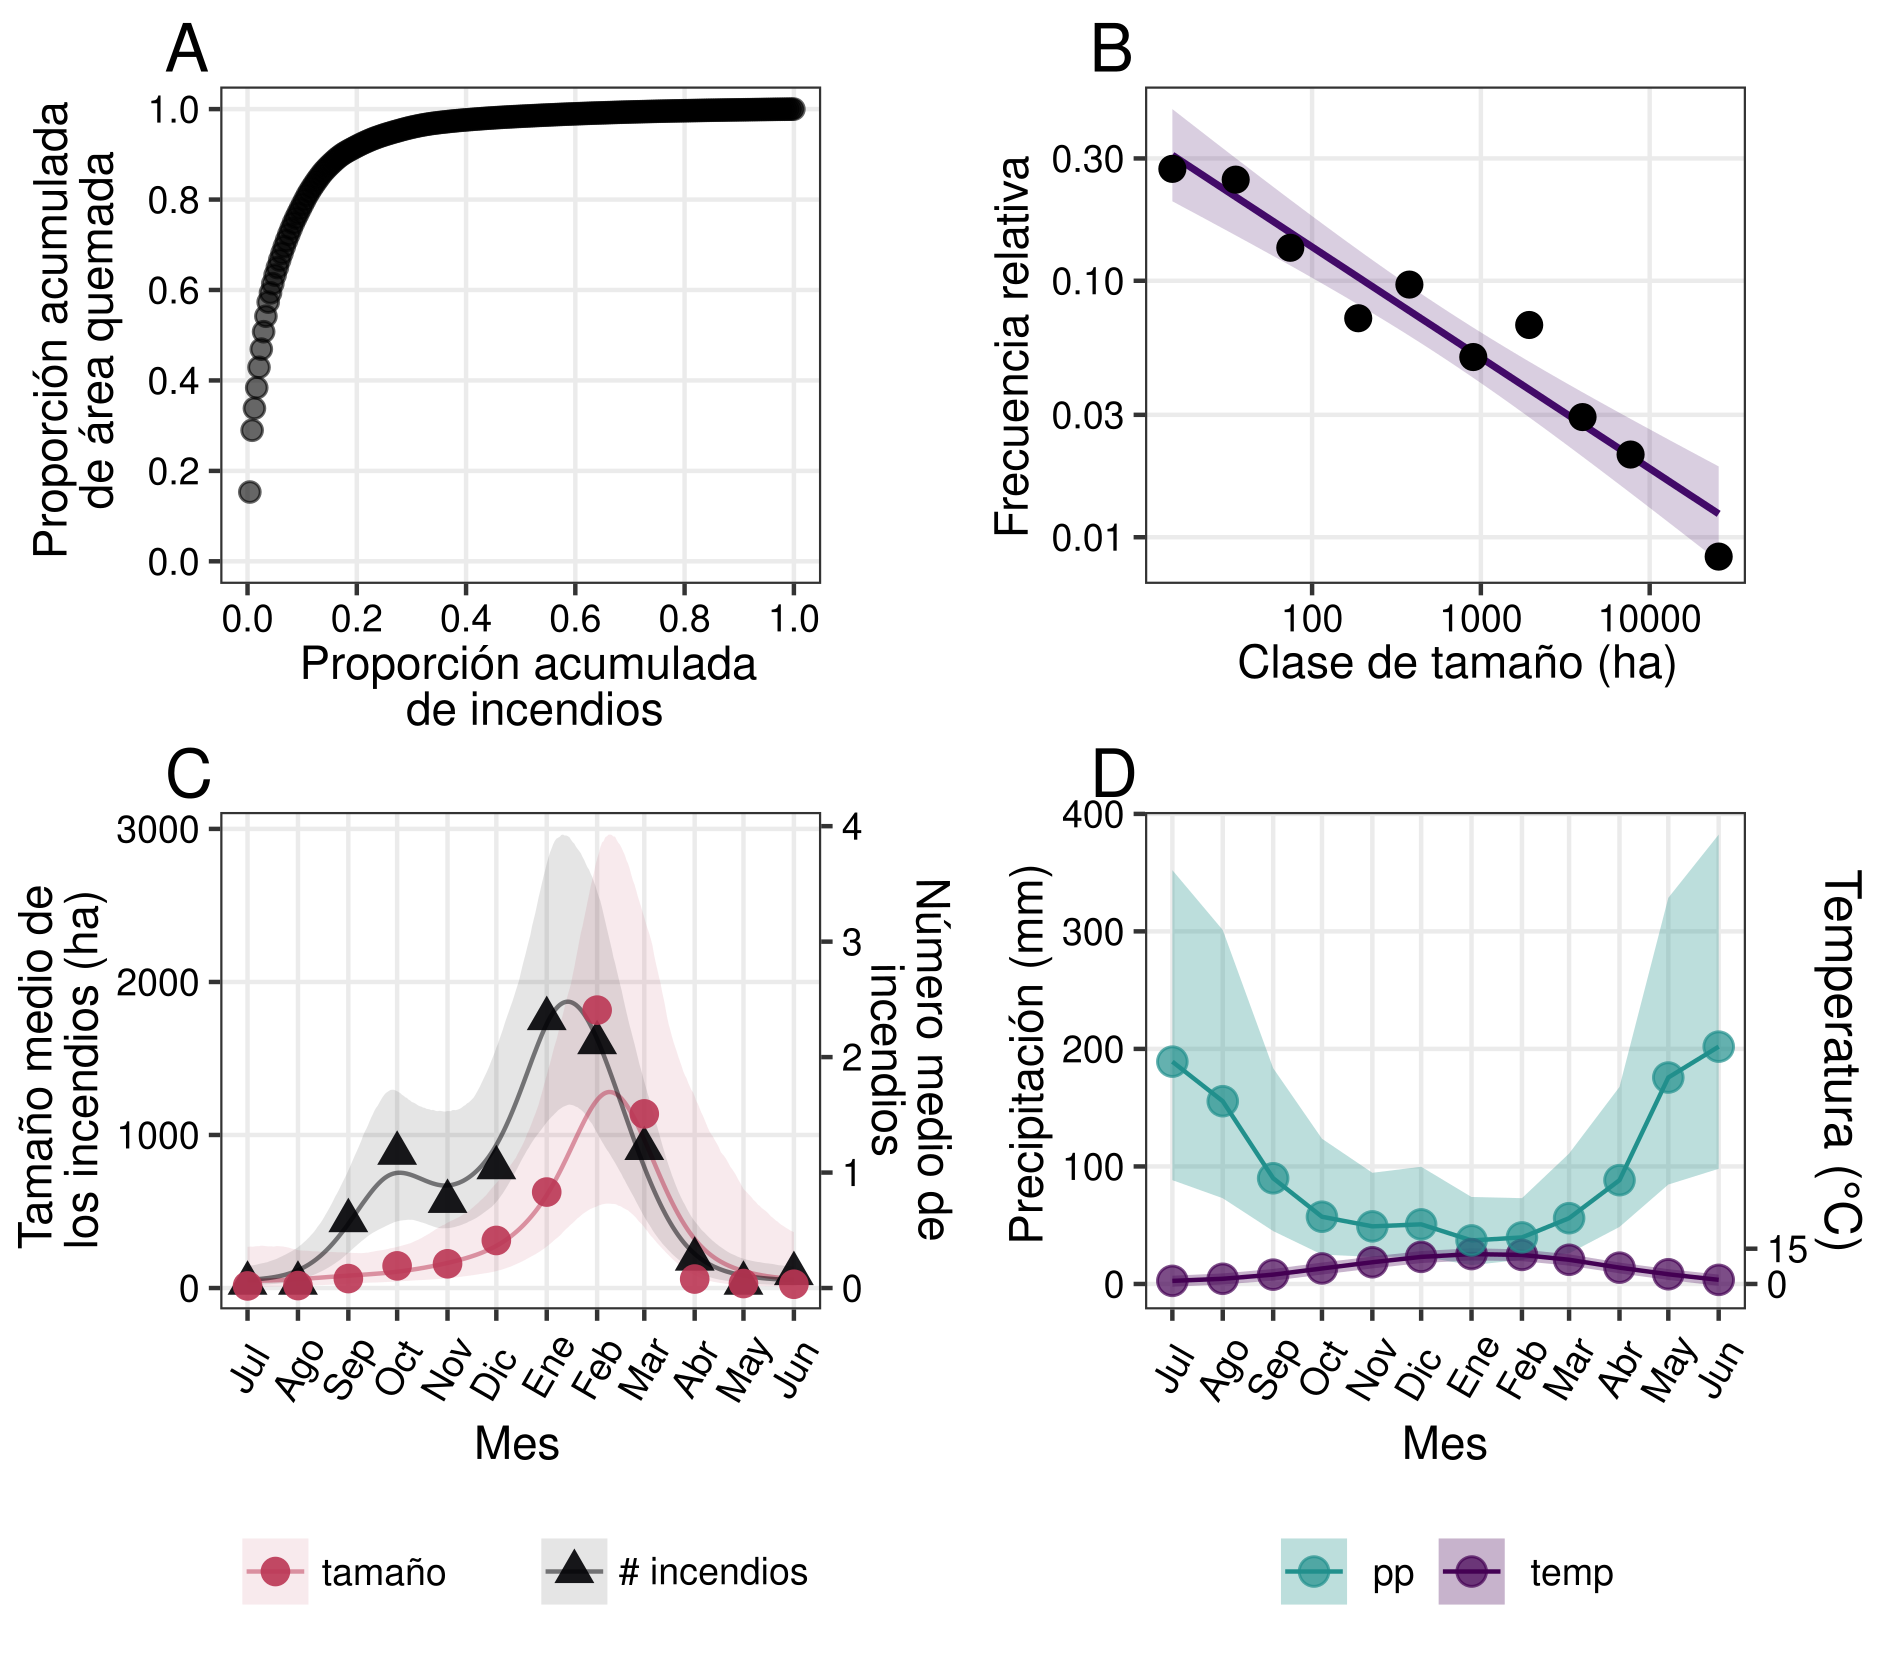
\includegraphics[width=16cm]{figuras/cap3/02) fire_regime.png}
    \caption[Distribución de tamaños y estacionalidad de incendios.]{(A) Proporción acumulada del área quemada en función de la proporción acumulada de incendios, ordenados de mayor a menor. (B) Frecuencia relativa de incendios por clase de tamaño (ambas variables en escala $\text{log}_{10}$). La línea y la banda muestran la media y el intervalo de confianza (IC) del 95 \% de una regresión lineal. (C) Tamaño promedio de los incendios y número de incendios por año y mes, promediados en los 24 años. Las curvas y bandas muestran la media y el IC del 95 \% estimados por los GAM, para un año promedio. (D) Precipitación y temperatura mensuales promedio, resumidas en todo el área de estudio con la media (puntos) y los percentiles 5 \% y 95 \% (bandas). Las líneas conectan los puntos solo para mejorar la visibilidad.} 
    \label{fig:cap3-02}
\end{figure}

\FloatBarrier

\subsection{Patrones temporales interanuales: incidencia del fuego en función de las variaciones climáticas}

Entre 1999 y 2022, la proporción anual promedio quemada en relación al área quemable fue del 0.25 \% (5400 ha), variando mayormente entre el 0.001 \% (21.24 ha) y el 0.78 \% (17144 ha), con un valor extremo del 2.04 \% (44578 ha) en 2015 (Fig.~\ref{fig:cap3-03}A). El número anual de incendios varió entre 1 y 28, con una media de 9.92. La proporción quemada anual y el número de incendios mostraron una ligera tendencia creciente con el tiempo, aunque con alta incertidumbre y elevados valores P (0.34 y 0.63, respectivamente; Tabla~\ref{tab:climate-ts}). Por el contrario, las variables climáticas mostraron claras tendencias hacia veranos más secos y cálidos, generalmente con valores P bajos (Tabla~\ref{tab:climate-ts}).

La proporción quemada anual y el número de incendios mostraron una variación clara en función de las variables climáticas, con valores de $\text{R}^2$ que oscilaron entre el 32 \% y el 60 \% (Fig.~\ref{fig:cap3-03}B). Ambas variables aumentaron con la temperatura, el déficit de presión de vapor y el FWI, y disminuyeron con la precipitación (Fig.~\ref{fig:cap3-03}B). La proporción quemada anual mostró una respuesta lineal a la temperatura, la precipitación y el FWI en escala logarítmica (lo que implica una respuesta exponencial en la escala original), pero el déficit de presión de vapor mostró un efecto de saturación (Fig.~\ref{fig:cap3-03}B). El número de incendios mostró una respuesta de saturación a todas las predictoras, excepto para el FWI, que produjo un efecto aproximadamente exponencial (Fig.~\ref{fig:cap3-03}B). Sin embargo, los efectos de saturación del déficit de presión de vapor sobre la proporción quemada anual (en $\text{log}_{10}$) y el número de incendios estuvieron fuertemente influenciados por el año 2022, que mostró el déficit de presión de vapor más alto, escasos incendios y una proporción quemada moderada (Fig.~\ref{fig:cap3-03}B).

\begin{figure}[htbp]
    \centering
    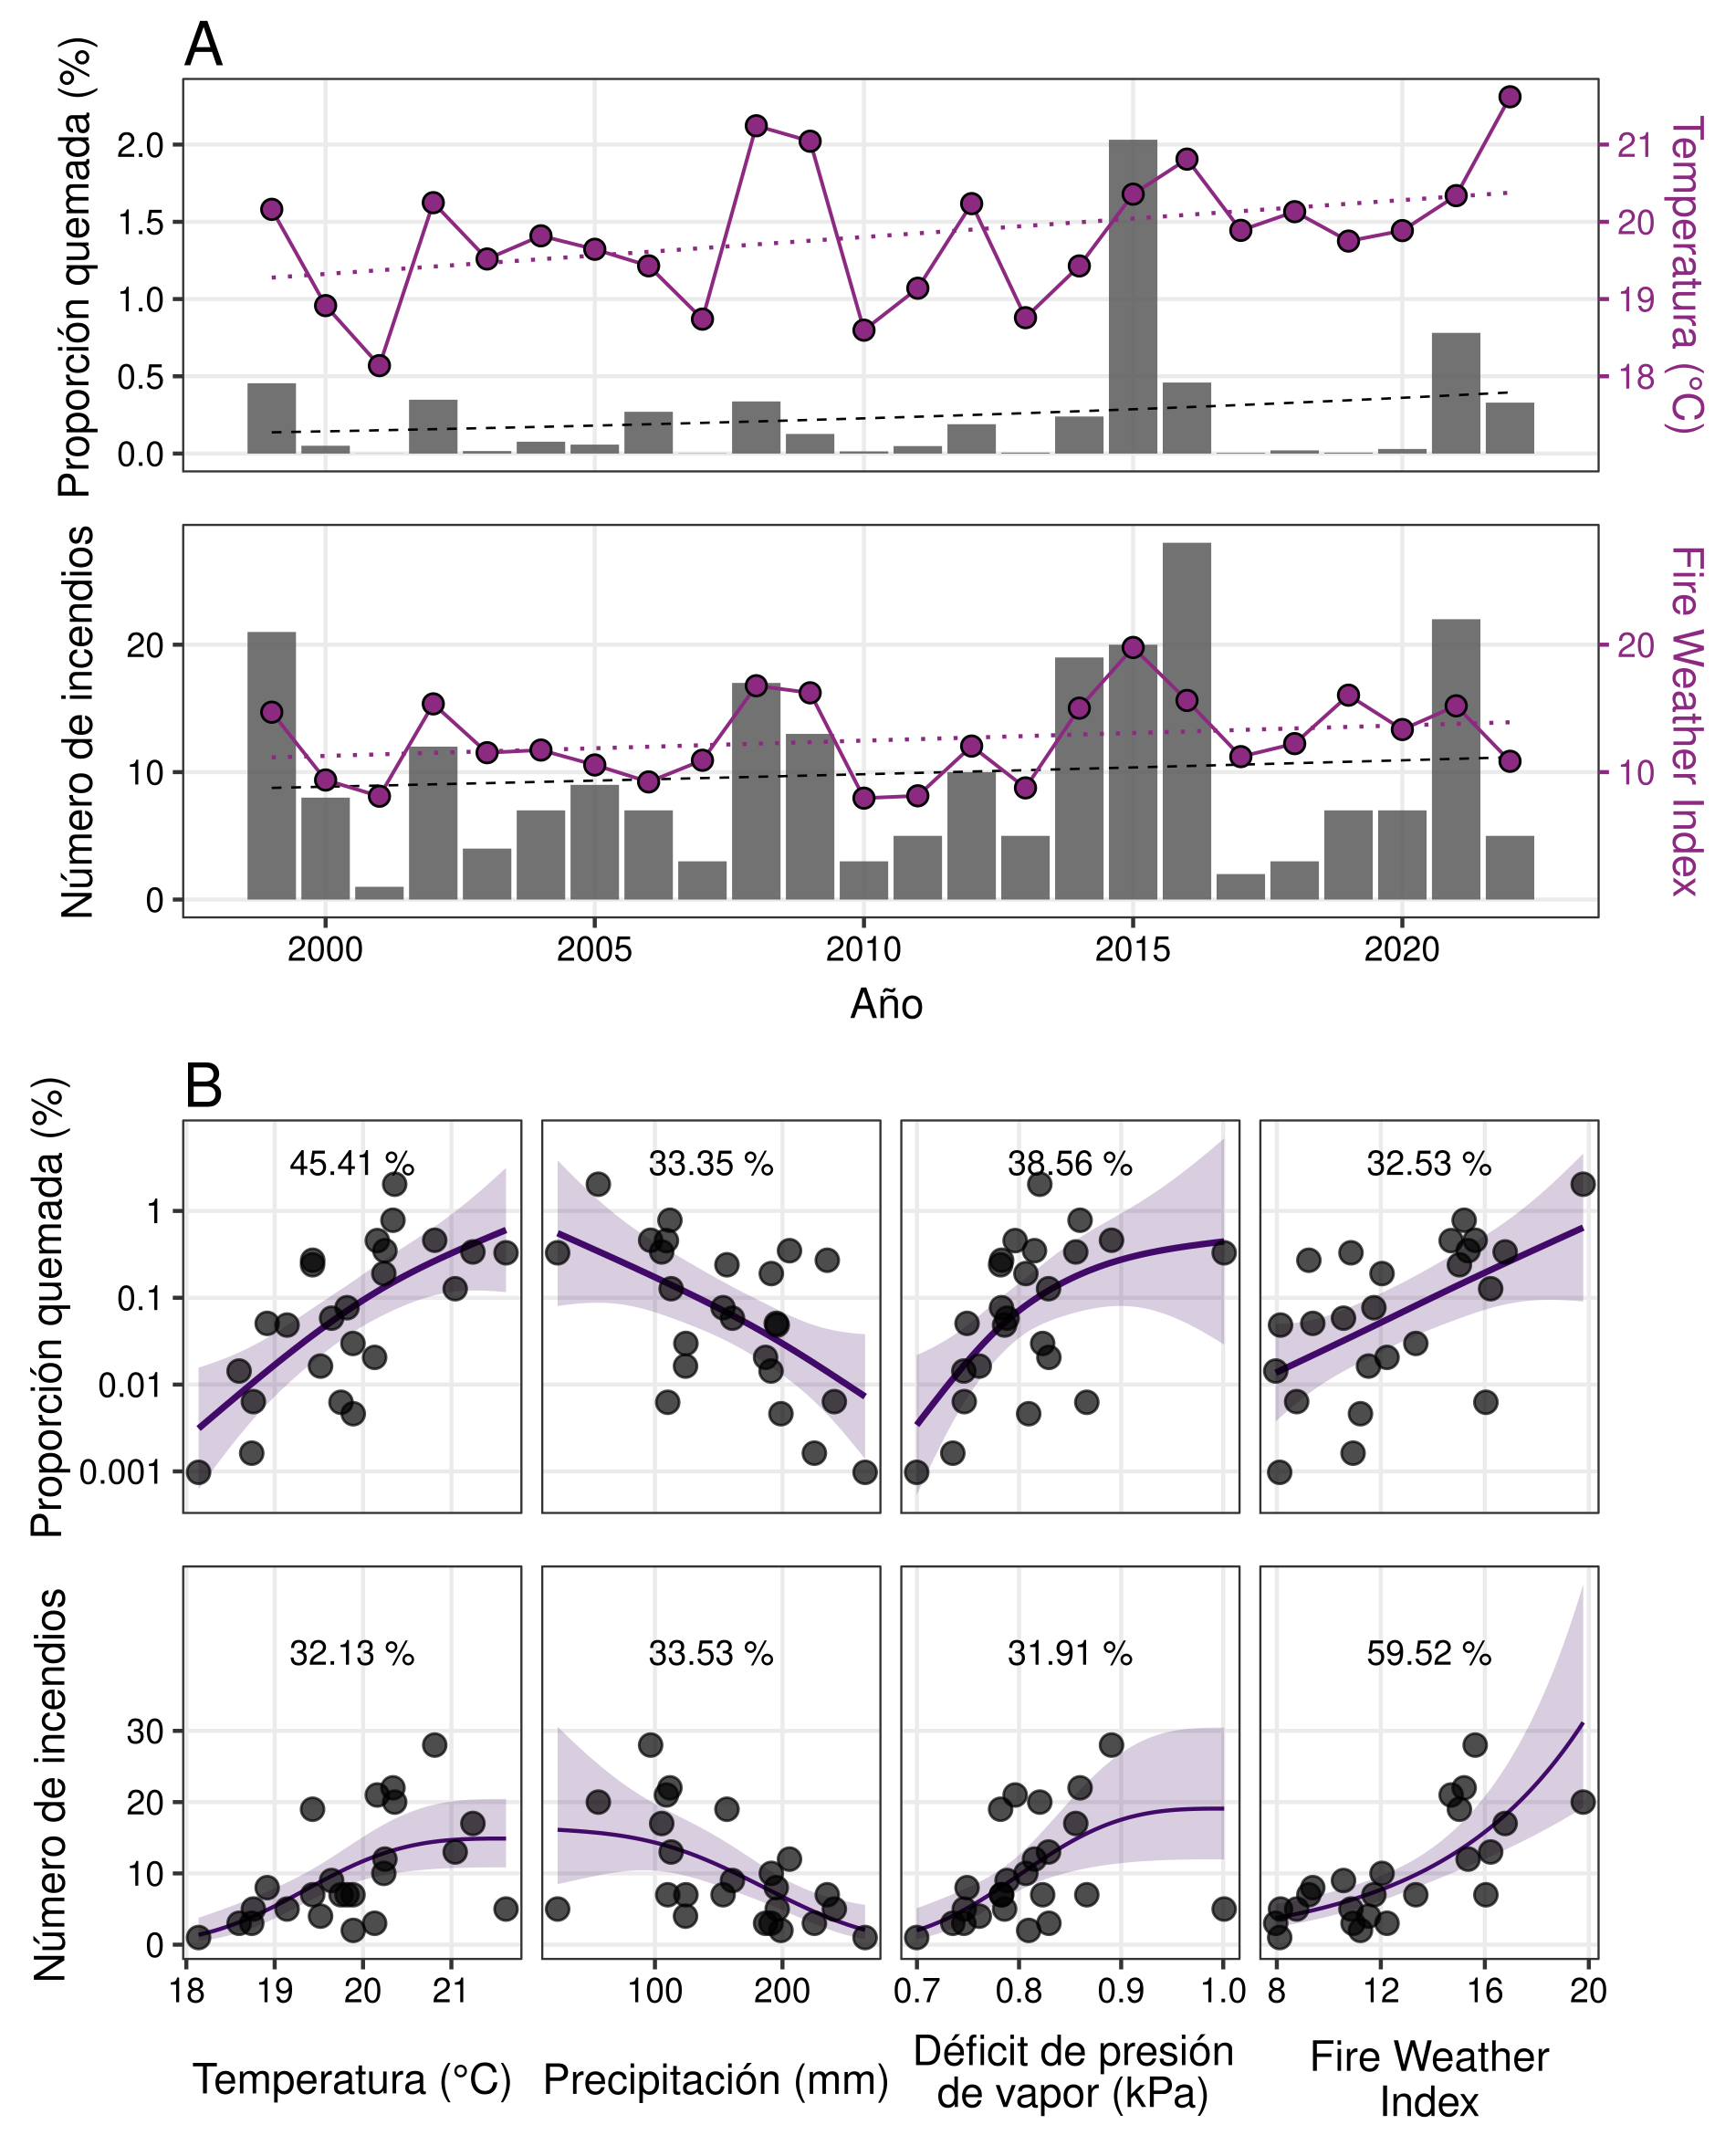
\includegraphics[width=16cm]{figuras/cap3/03) temporal_trends.png}
    \caption[Patrones temporales interanuales en la incidencia del fuego.]{(A) Proporción quemada anual del paisaje (arriba) y número de incendios $\ge 10$ ha (abajo) por año (barras), junto con la serie temporal de la variable climática con mayor efecto (temperatura y Fire Weather Index, respectivamente; puntos y línea). Las líneas punteadas y discontinuas muestran la media predicha de los modelos de tendencia interanual ajustados a cada variable. (B) Proporción quemada anual (arriba, en escala $\text{log}_{10}$) y número de incendios $\ge 10$ ha (abajo) en función de variables climáticas por año, promediadas entre diciembre y marzo. Las curvas y bandas muestran las medias estimadas por los GAM con restricciones de forma y sus IC del 95 \%. Los números dentro de los paneles muestran los valores de $\text{R}^2$ bayesiano (\%;  \citealt{gelman_r-squared_2019}).} 
    \label{fig:cap3-03}
\end{figure}

\begin{table}[ht]
\centering
\caption[Tendencias temporales en incidencia del fuego y variables climáticas.]{Proporción quemada y número de incendios por año y variables climáticas (promediadas durante la temporada de incendios) en función del tiempo (con el año como única predictora). Los modelos de proporción quemada y número de incendios fueron ajustados con un enlace logarítmico, por lo que $\exp{(\beta)}$ representa el factor de aumento anual. Las pendientes restantes son las tasas de cambio anual en la escala de la respuesta (enlace identidad). Los valores de $\text{R}^2$ bayesiano se muestran en la última columna \citep{gelman_r-squared_2019}.}
\label{tab:climate-ts}
\begin{tabular}{lccccc}
\toprule
Variable respuesta & $\beta$ & Error estándar & t & P & $\text{R}^2$ (\%) \\
\midrule
Proporción quemada (\%)           & 0.046   & 0.047 & 0.976  & 0.340 & 8.616  \\
Número de incendios               & 0.011   & 0.022 & 0.491  & 0.624 & 1.032  \\
Temperatura ($^\circ$C)           & 0.048   & 0.024 & 1.992  & 0.059 & 14.716 \\
Precipitación (mm)                & -3.635  & 1.658 & -2.192 & 0.039 & 17.286 \\
Déficit de presión de vapor (kPa) & 0.006   & 0.001 & 3.924  & 0.001 & 40.098 \\
Fire Weather Index                & 0.120   & 0.094 & 1.273  & 0.216 & 6.582  \\
\bottomrule
\end{tabular}
\end{table}

\FloatBarrier

\subsection{Patrones espaciales: efectos de la vegetación, topografía, precipitación e influencia humana}

En el modelo ambiental, donde no se consideró el tipo de vegetación, la altitud y la precipitación fueron los controles físicos más fuertes sobre la probabilidad de quema, que fue mayor en áreas de baja altitud y precipitación (Fig.~\ref{fig:cap3-04}A.1 y \ref{fig:cap3-05}A.1). La probabilidad de quema también aumentó en pendientes pronunciadas orientadas al norte y disminuyó ligeramente con la posición topográfica (Fig.~\ref{fig:cap3-04}.1). Sin embargo, estas variables mostraron efectos menores. El NDVI mostró un efecto unimodal, con la mayor probabilidad de quema en valores intermedios (Fig.~\ref{fig:cap3-05}B.1). Las distancias a poblados y a caminos aumentaron considerablemente la probabilidad de quema, aunque sus efectos no se diferenciaron del azar (Fig.~\ref{fig:cap3-05}D.1).

En el modelo conjunto, que permite predecir los efectos de las variables ambientales por separado para cada tipo de vegetación, los efectos de la altitud y la pendiente se mantuvieron cualitativamente similares a los del modelo ambiental, pero variaron en magnitud. En la mayoría de los casos, el modelo ambiental mostró un tamaño de efecto intermedio. Esto sugiere que los efectos de la altitud y la pendiente se mantienen dentro de los tipos de vegetación, indicando que afectan el fuego directamente y no por su asociación con los tipos de vegetación. En los bosques húmedos y secos, la altitud mostró los mayores efectos sobre la probabilidad de quema, aunque con incertidumbre considerable en los bosques secos (P = 0.386). En los bosques subalpinos y matorrales, la altitud mostró efectos menores y esperables por azar (P = 0.776; Fig.~\ref{fig:cap3-04}A). El efecto positivo de la pendiente fue mayor en los matorrales y casi nulo en los pastizales (Fig.~\ref{fig:cap3-04}B). A diferencia de la altitud y la pendiente, el efecto de la orientación fue mayor en el modelo ambiental que dentro de los tipos de vegetación (modelo conjunto, Fig.~\ref{fig:cap3-04}C), lo que indica que la orientación afecta la probabilidad de quema al controlar la distribución de los tipos de vegetación (Fig.~\ref{fig:cap3-S01}). El efecto de la posición topográfica varió considerablemente entre los tipos de vegetación. Fue grande y positivo en los bosques húmedos y secos, aunque esperable por azar (P = 0.258). En los bosques subalpinos y pastizales, el efecto de la posición topográfica fue insignificante, y en los matorrales, fue pequeño y negativo (Fig.~\ref{fig:cap3-04}D).

La precipitación mostró un patrón similar al de la orientación: la disminución en la probabilidad de quema con la precipitación observada en el modelo ambiental se desdibujó en el modelo conjunto, donde se incluyeron los tipos de vegetación (Fig.~\ref{fig:cap3-05}A). Esto indica que el efecto de la precipitación observado cuando no se considera el tipo de vegetación se debe principalmente al recambio del  tipo de vegetación a lo largo del gradiente de precipitación (Fig.~\ref{fig:cap3-S01}). Dentro de los tipos de vegetación, el efecto de la precipitación solo fue claro en los bosques subalpinos, pero mostró una magnitud pequeña. En los bosques secos, el efecto fue mayor que en el modelo ambiental, pero esperable por azar. El NDVI mostró un efecto unimodal, evidente tanto en el modelo ambiental como dentro de la mayoría de los tipos de vegetación en el modelo conjunto (Fig.~\ref{fig:cap3-05}B). Este efecto fue mayor en los bosques húmedos, intermedio en los bosques subalpinos y menor en los pastizales y matorrales. En los bosques secos, el efecto del NDVI fue grande y negativo, pero esperable por azar (P = 0.424).

En el modelo conjunto, la distancia a caminos y a poblados mostró efectos positivos y de gran magnitud en algunos tipos de vegetación. Sin embargo, al igual que en el modelo ambiental, en ningún caso estos efectos se diferenciaron
estadísticamente del azar (Fig.~\ref{fig:cap3-05}D).

Los tipos de vegetación mostraron claras diferencias en la probabilidad de quema en el modelo de vegetación, que no incluyó variables ambientales (Fig.~\ref{fig:cap3-06}A). La probabilidad de quema fue mayor en los bosques secos, matorrales y plantaciones, y menor en los bosques subalpinos y praderas antrópicas. Sin embargo, las altas y bajas probabilidades de quema de las plantaciones y praderas antrópicas no se diferenciaron claramente del azar. Los bosques húmedos y pastizales mostraron probabilidades de quema intermedias (Fig.~\ref{fig:cap3-06}A).

Cuando se compararon los tipos de vegetación bajo las mismas condiciones ambientales utilizando el modelo conjunto, aún mostraron variaciones en la probabilidad de quema, pero con patrones diferentes respecto al modelo de vegetación, y con tamaños de efecto más pequeños y con mayor incertidumbre (comparar Fig.~\ref{fig:cap3-06}A con \ref{fig:cap3-06}C). Esto indica que las probabilidades de quema estimadas por el modelo de vegetación están influenciadas parcialmente por las condiciones ambientales contrastantes donde cada tipo de vegetación es más frecuente. Aunque los bosques subalpinos mostraron la menor probabilidad de quema cuando no se consideraron las variables ambientales (Fig.~\ref{fig:cap3-06}A), presentaron valores más cercanos al promedio cuando se compararon a iguales condiciones. Su probabilidad de quema fue mayor que en los bosques húmedos, similar a la de los pastizales y menor que en los matorrales (Fig.~\ref{fig:cap3-06}C.1 y \ref{fig:cap3-06}C.2). Los bosques secos, con la mayor probabilidad de quema en el modelo de vegetación, mostraron valores más bajos que los matorrales y similares a los pastizales cuando se compararon a iguales condiciones (Fig.~\ref{fig:cap3-06}C.3 y \ref{fig:cap3-06}C.4). Los bosques húmedos, con una probabilidad intermedia en el modelo de vegetación, mostraron el valor más bajo cuando se compararon a alta altitud, y un valor intermedio a baja altitud (Fig.~\ref{fig:cap3-06}C.2 y \ref{fig:cap3-06}C.4). Los matorrales mostraron la mayor probabilidad de quema bajo todas las condiciones, aunque con baja precipitación y altitud, los bosques secos y pastizales presentaron valores similares (Fig.~\ref{fig:cap3-06}C.3). Además, sus diferencias respecto al promedio mostraron valores P mayores que en el modelo de vegetación.

El modelo conjunto mostró el mayor poder explicativo ($\text{R}^2 = 12.73$ \%), seguido por el modelo ambiental ($\text{R}^2 = 8.36$ \%) y el modelo de vegetación ($\text{R}^2 = 1.51$ \%; Tabla~\ref{tab:cap3-spat-models}).

\begin{figure}[htbp]
    \centering
    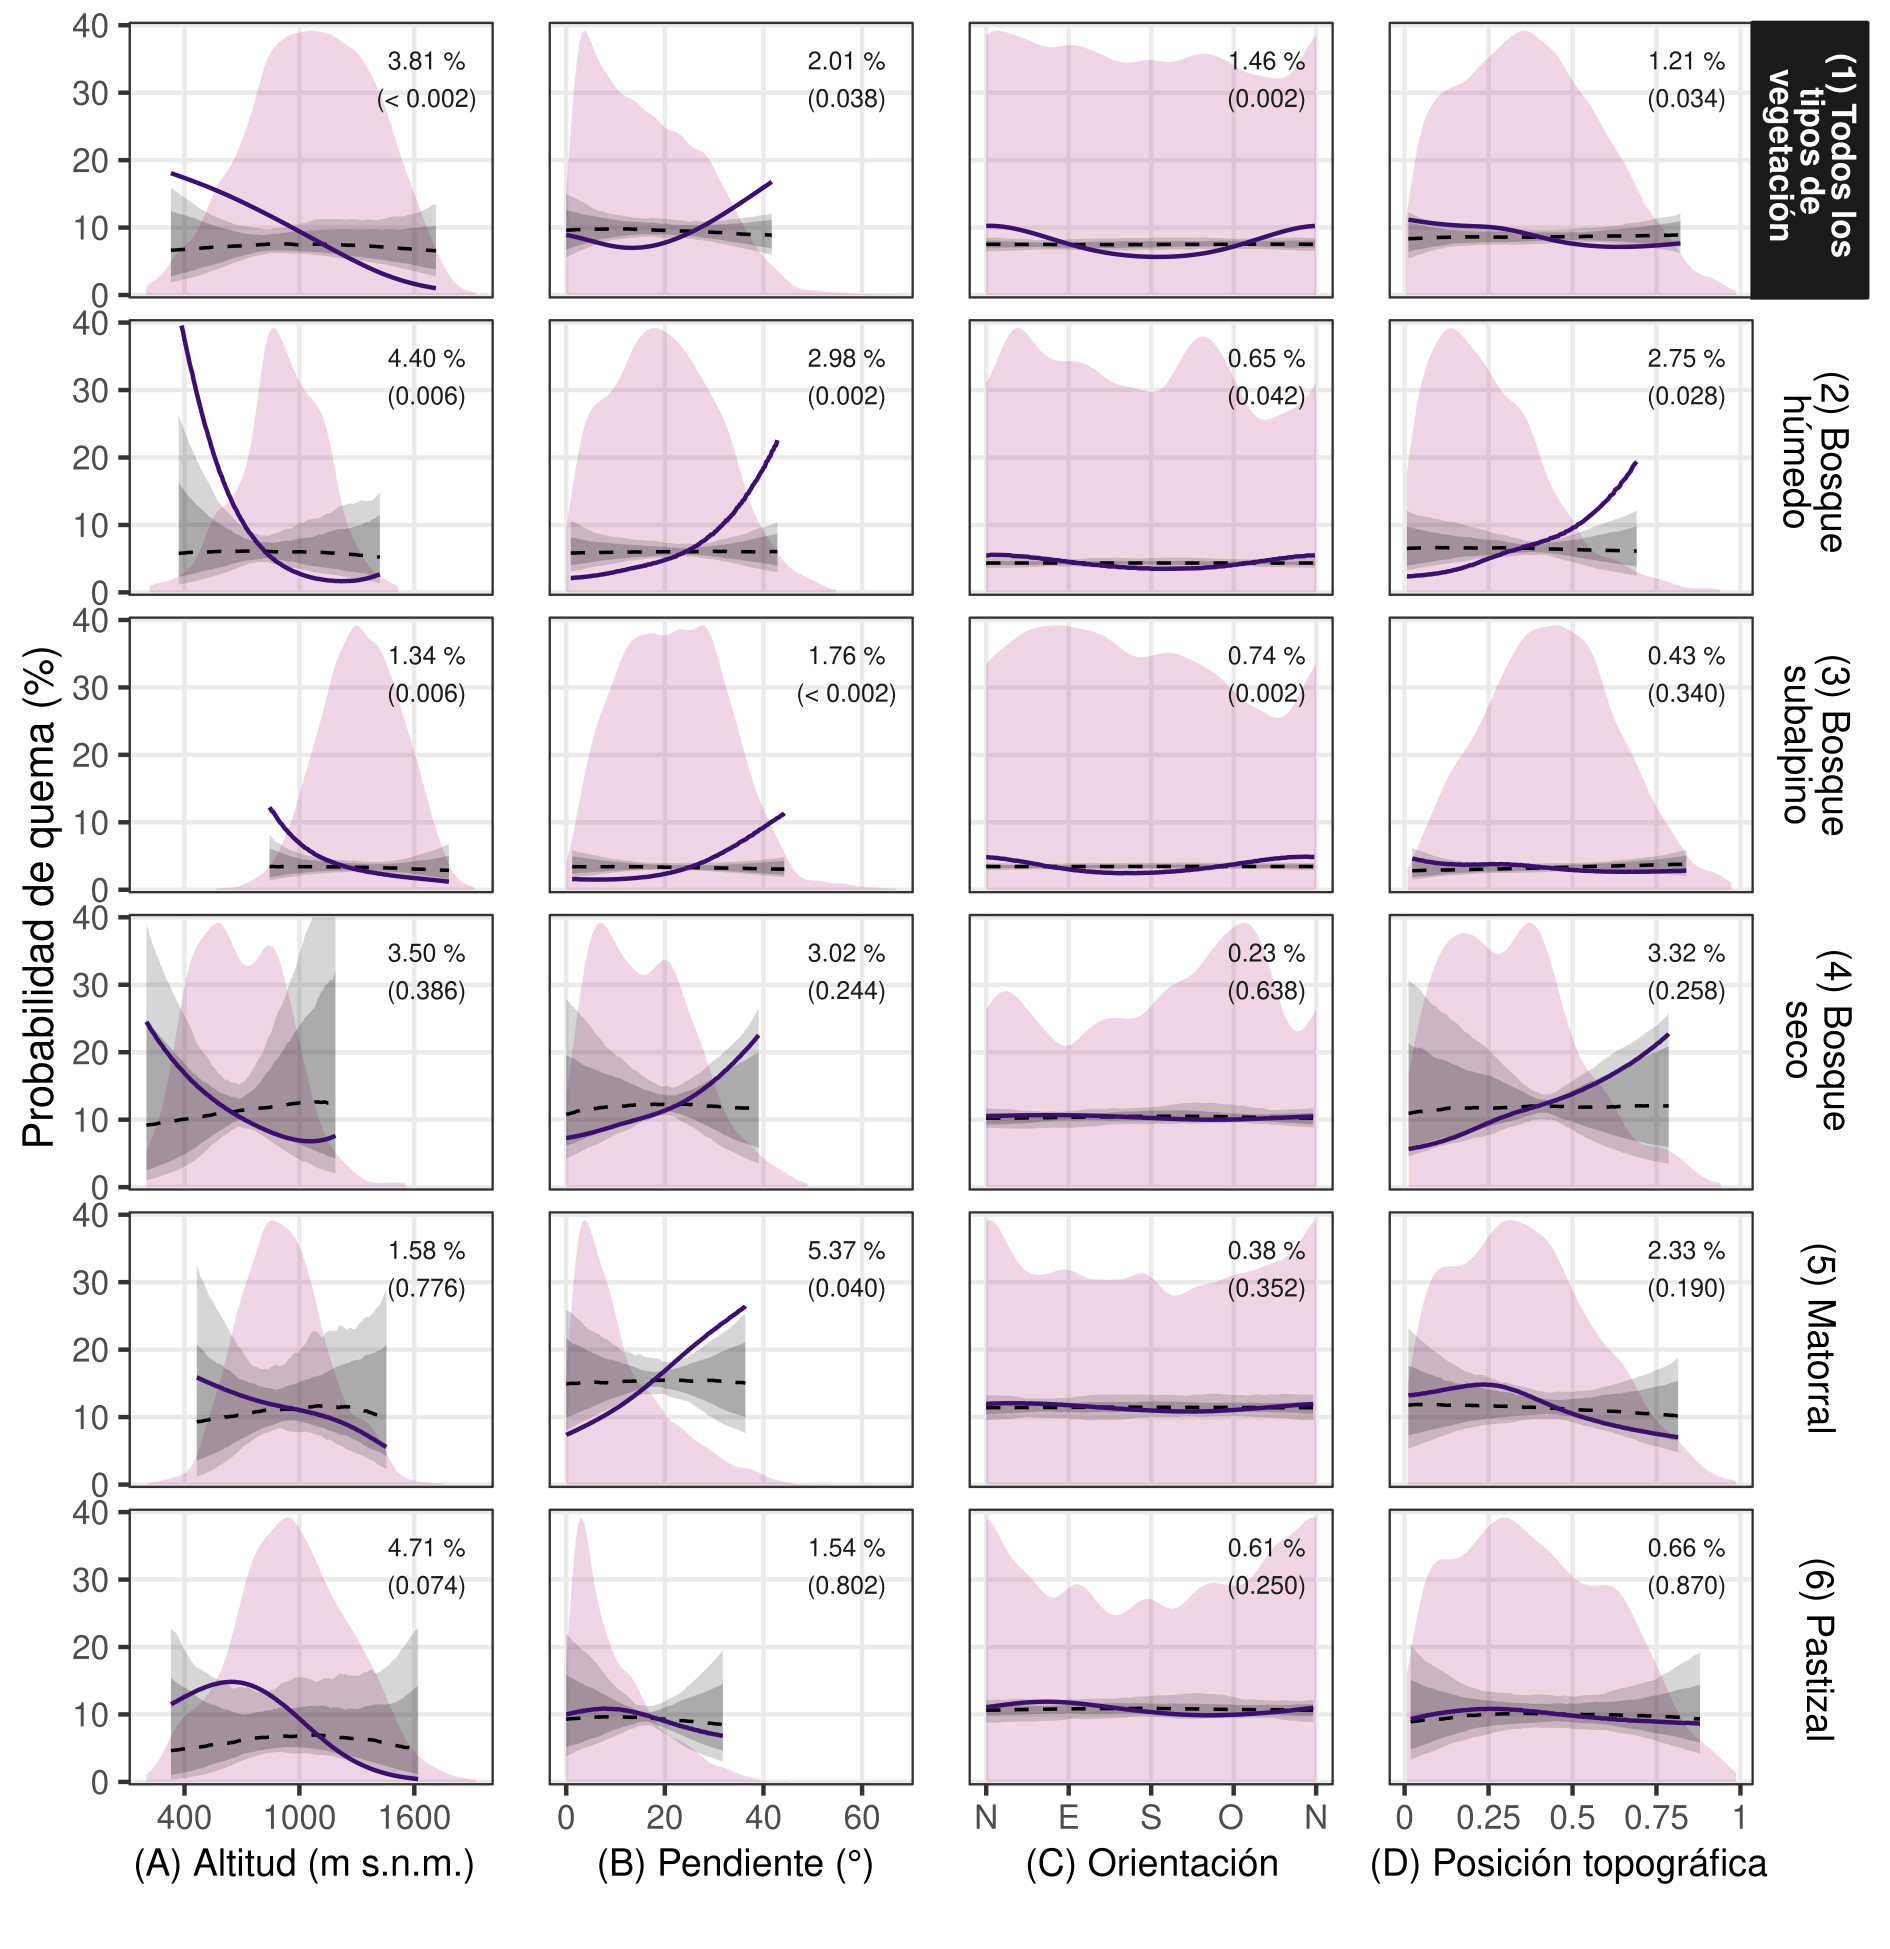
\includegraphics[width=16cm]{figuras/cap3/04) env_topo.png}
    \caption[Probabilidad de quema en función de variables topográficas.]{Probabilidad de quema en función de variables topográficas, predicha por el modelo ambiental, donde no se incluyó el tipo de vegetación (primera fila), y por el modelo conjunto, que incluye el tipo de vegetación (filas dos a seis). La línea sólida muestra la predicción de los modelos ajustados a los datos observados, mientras que las bandas grises y la línea discontinua muestran la distribución de la misma predicción obtenida a partir de modelos ajustados a datos aleatorizados (mediana e intervalos centrales de colas iguales con 80 \% y 95 \% de probabilidad). Las predicciones fueron calculadas a lo largo del intervalo de máxima densidad del 98 \% de cada predictora. Las sombras rosas muestran la distribución de la variable predictora. Los porcentajes dentro de los paneles indican el tamaño del efecto de cada predictora, con su correspondiente valor P.} 
    \label{fig:cap3-04}
\end{figure}

\begin{figure}[htbp]
    \centering
    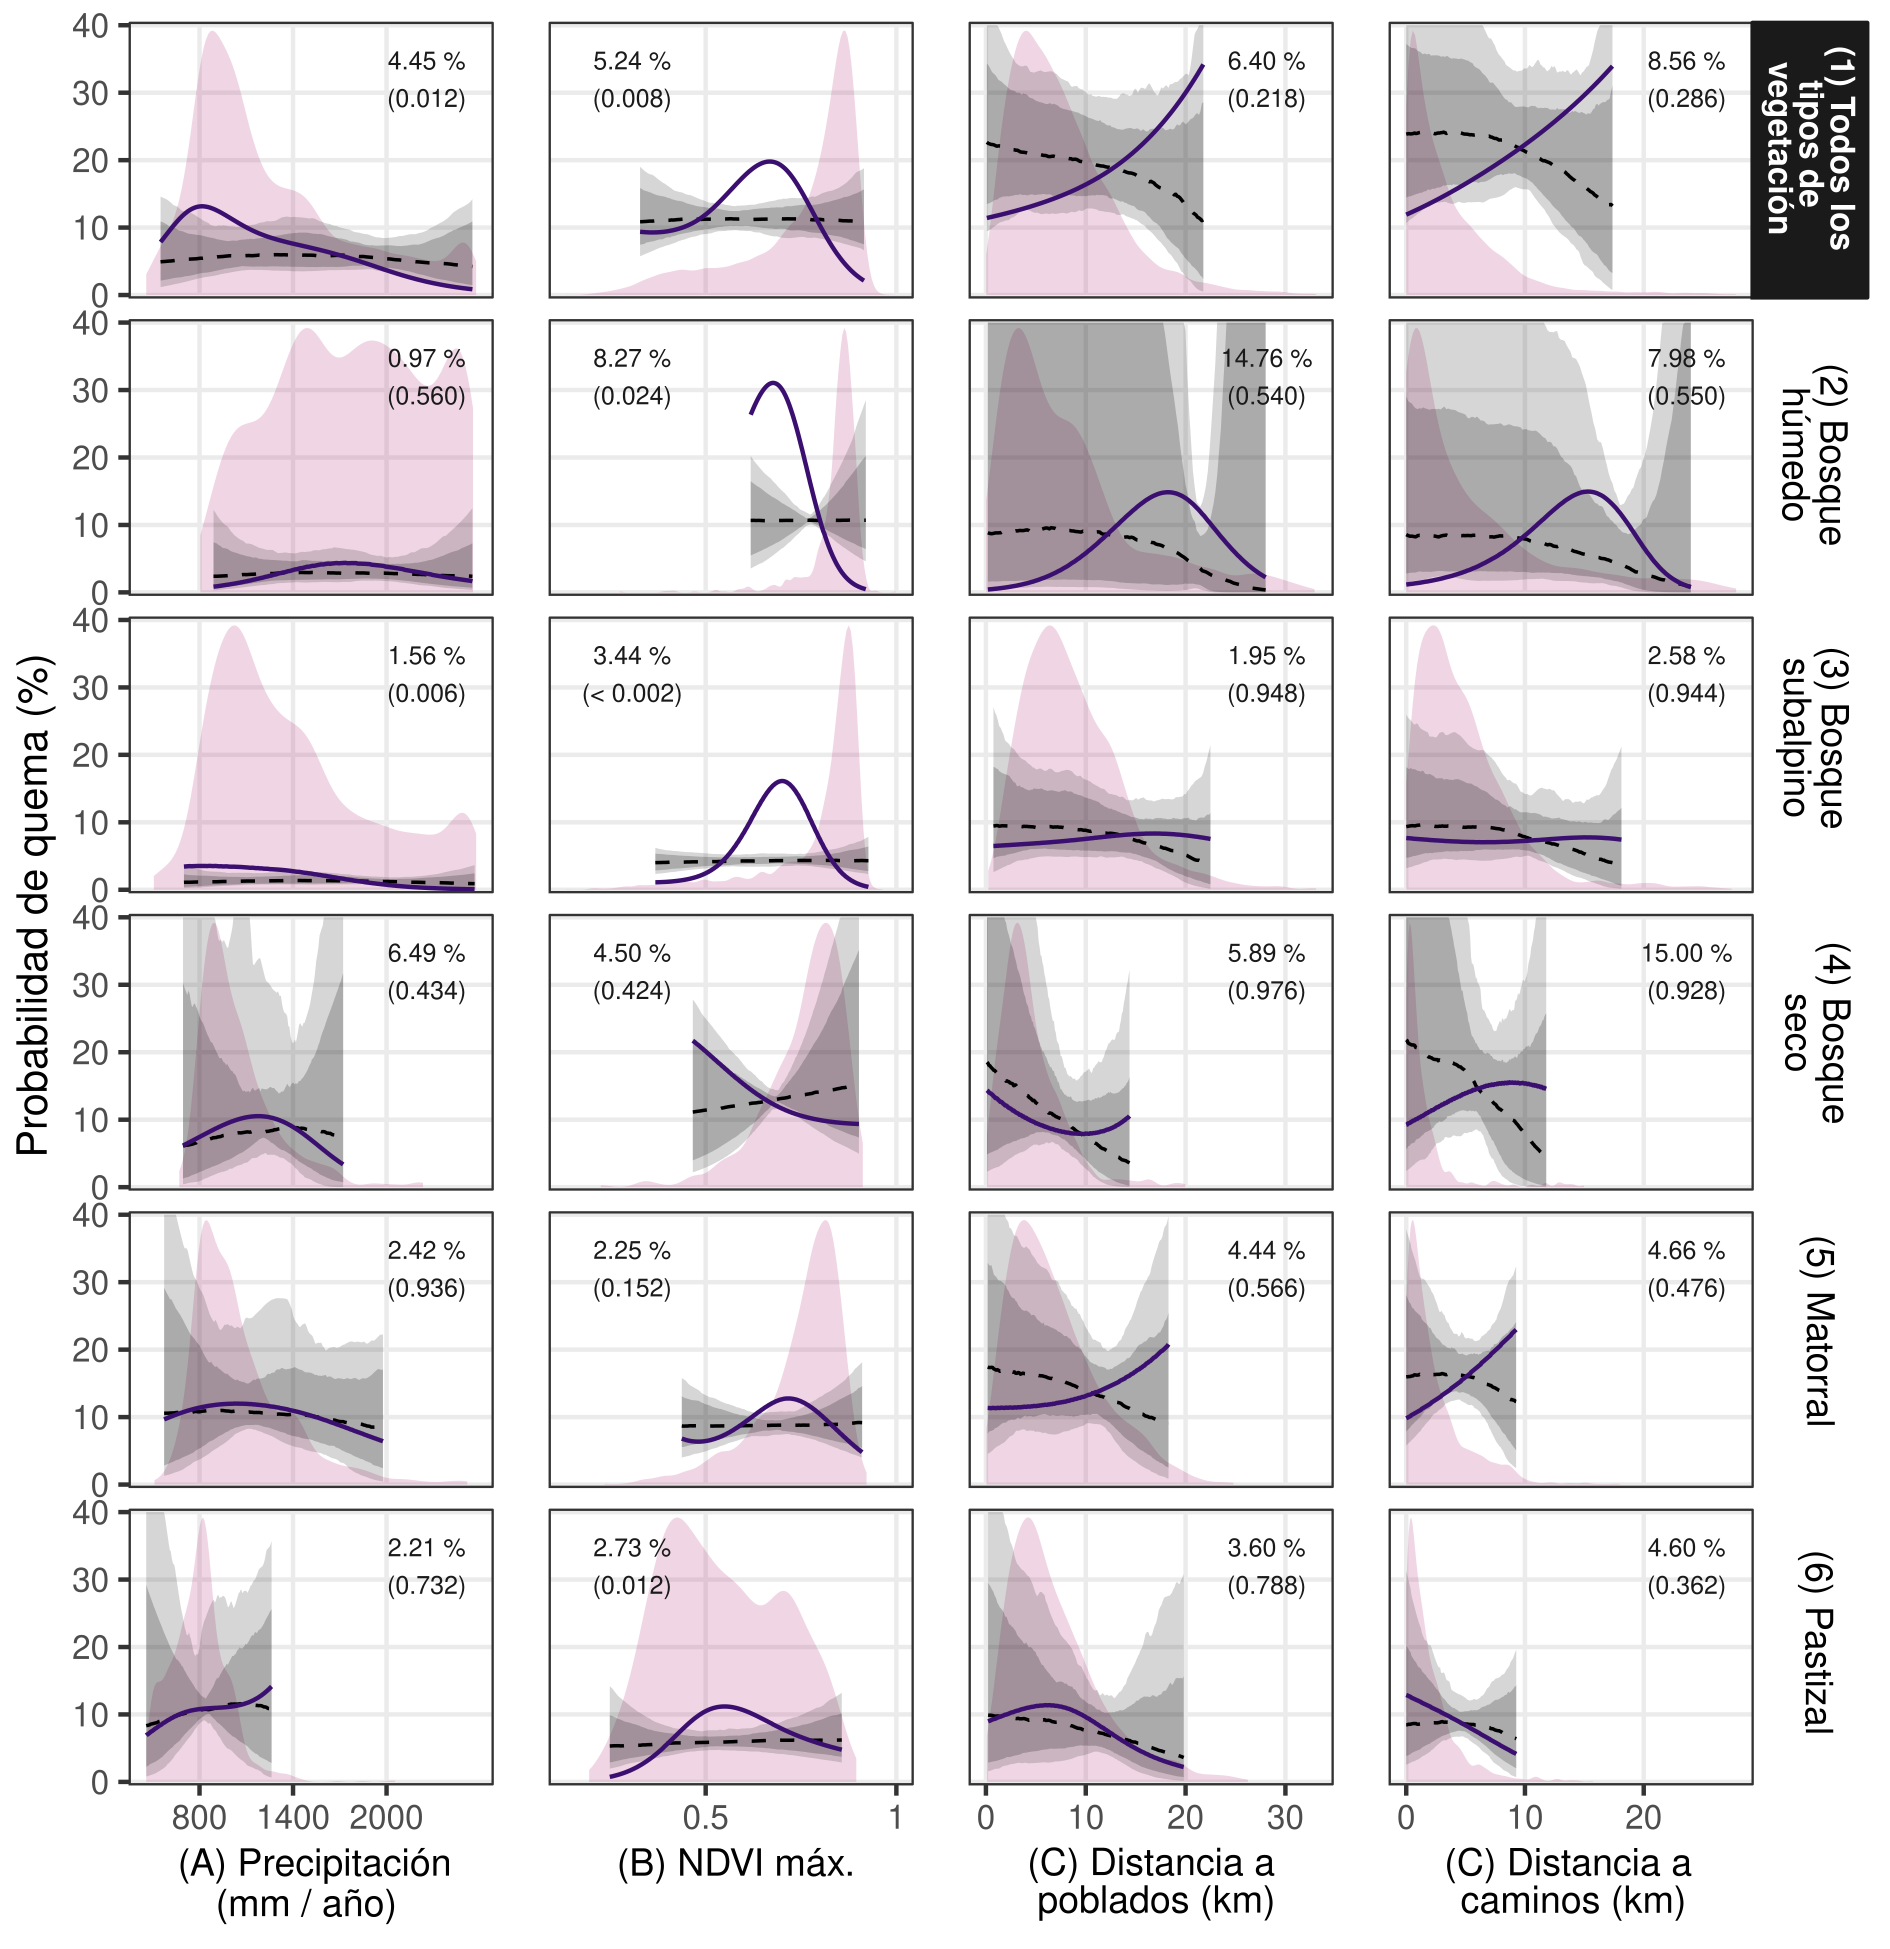
\includegraphics[width=16cm]{figuras/cap3/05) env_pp.png}
    \caption[Probabilidad de quema en función de la precipitación, el NDVI y la distancia a caminos y a poblados.]{Probabilidad de quema en función de la precipitación, el NDVI y la distancia a caminos y a poblados, predicha por el modelo ambiental, donde no se incluyó el tipo de vegetación (primera fila), y por el modelo conjunto, que incluye el tipo de vegetación (filas dos a seis). La línea sólida muestra la predicción de los modelos ajustados a los datos observados, mientras que las bandas grises y la línea discontinua muestran la distribución de la misma predicción obtenida a partir de modelos ajustados a datos aleatorizados (mediana e intervalos centrales de colas iguales con 80 \% y 95 \% de probabilidad). Las predicciones fueron calculadas a lo largo del intervalo de máxima densidad del 98 \% de cada predictora. Las sombras rosas muestran la distribución de la variable predictora. Los porcentajes dentro de los paneles indican el tamaño del efecto de cada predictora, con su correspondiente valor P.} 
    \label{fig:cap3-05}
\end{figure}

\begin{figure}[htbp]
    \centering
    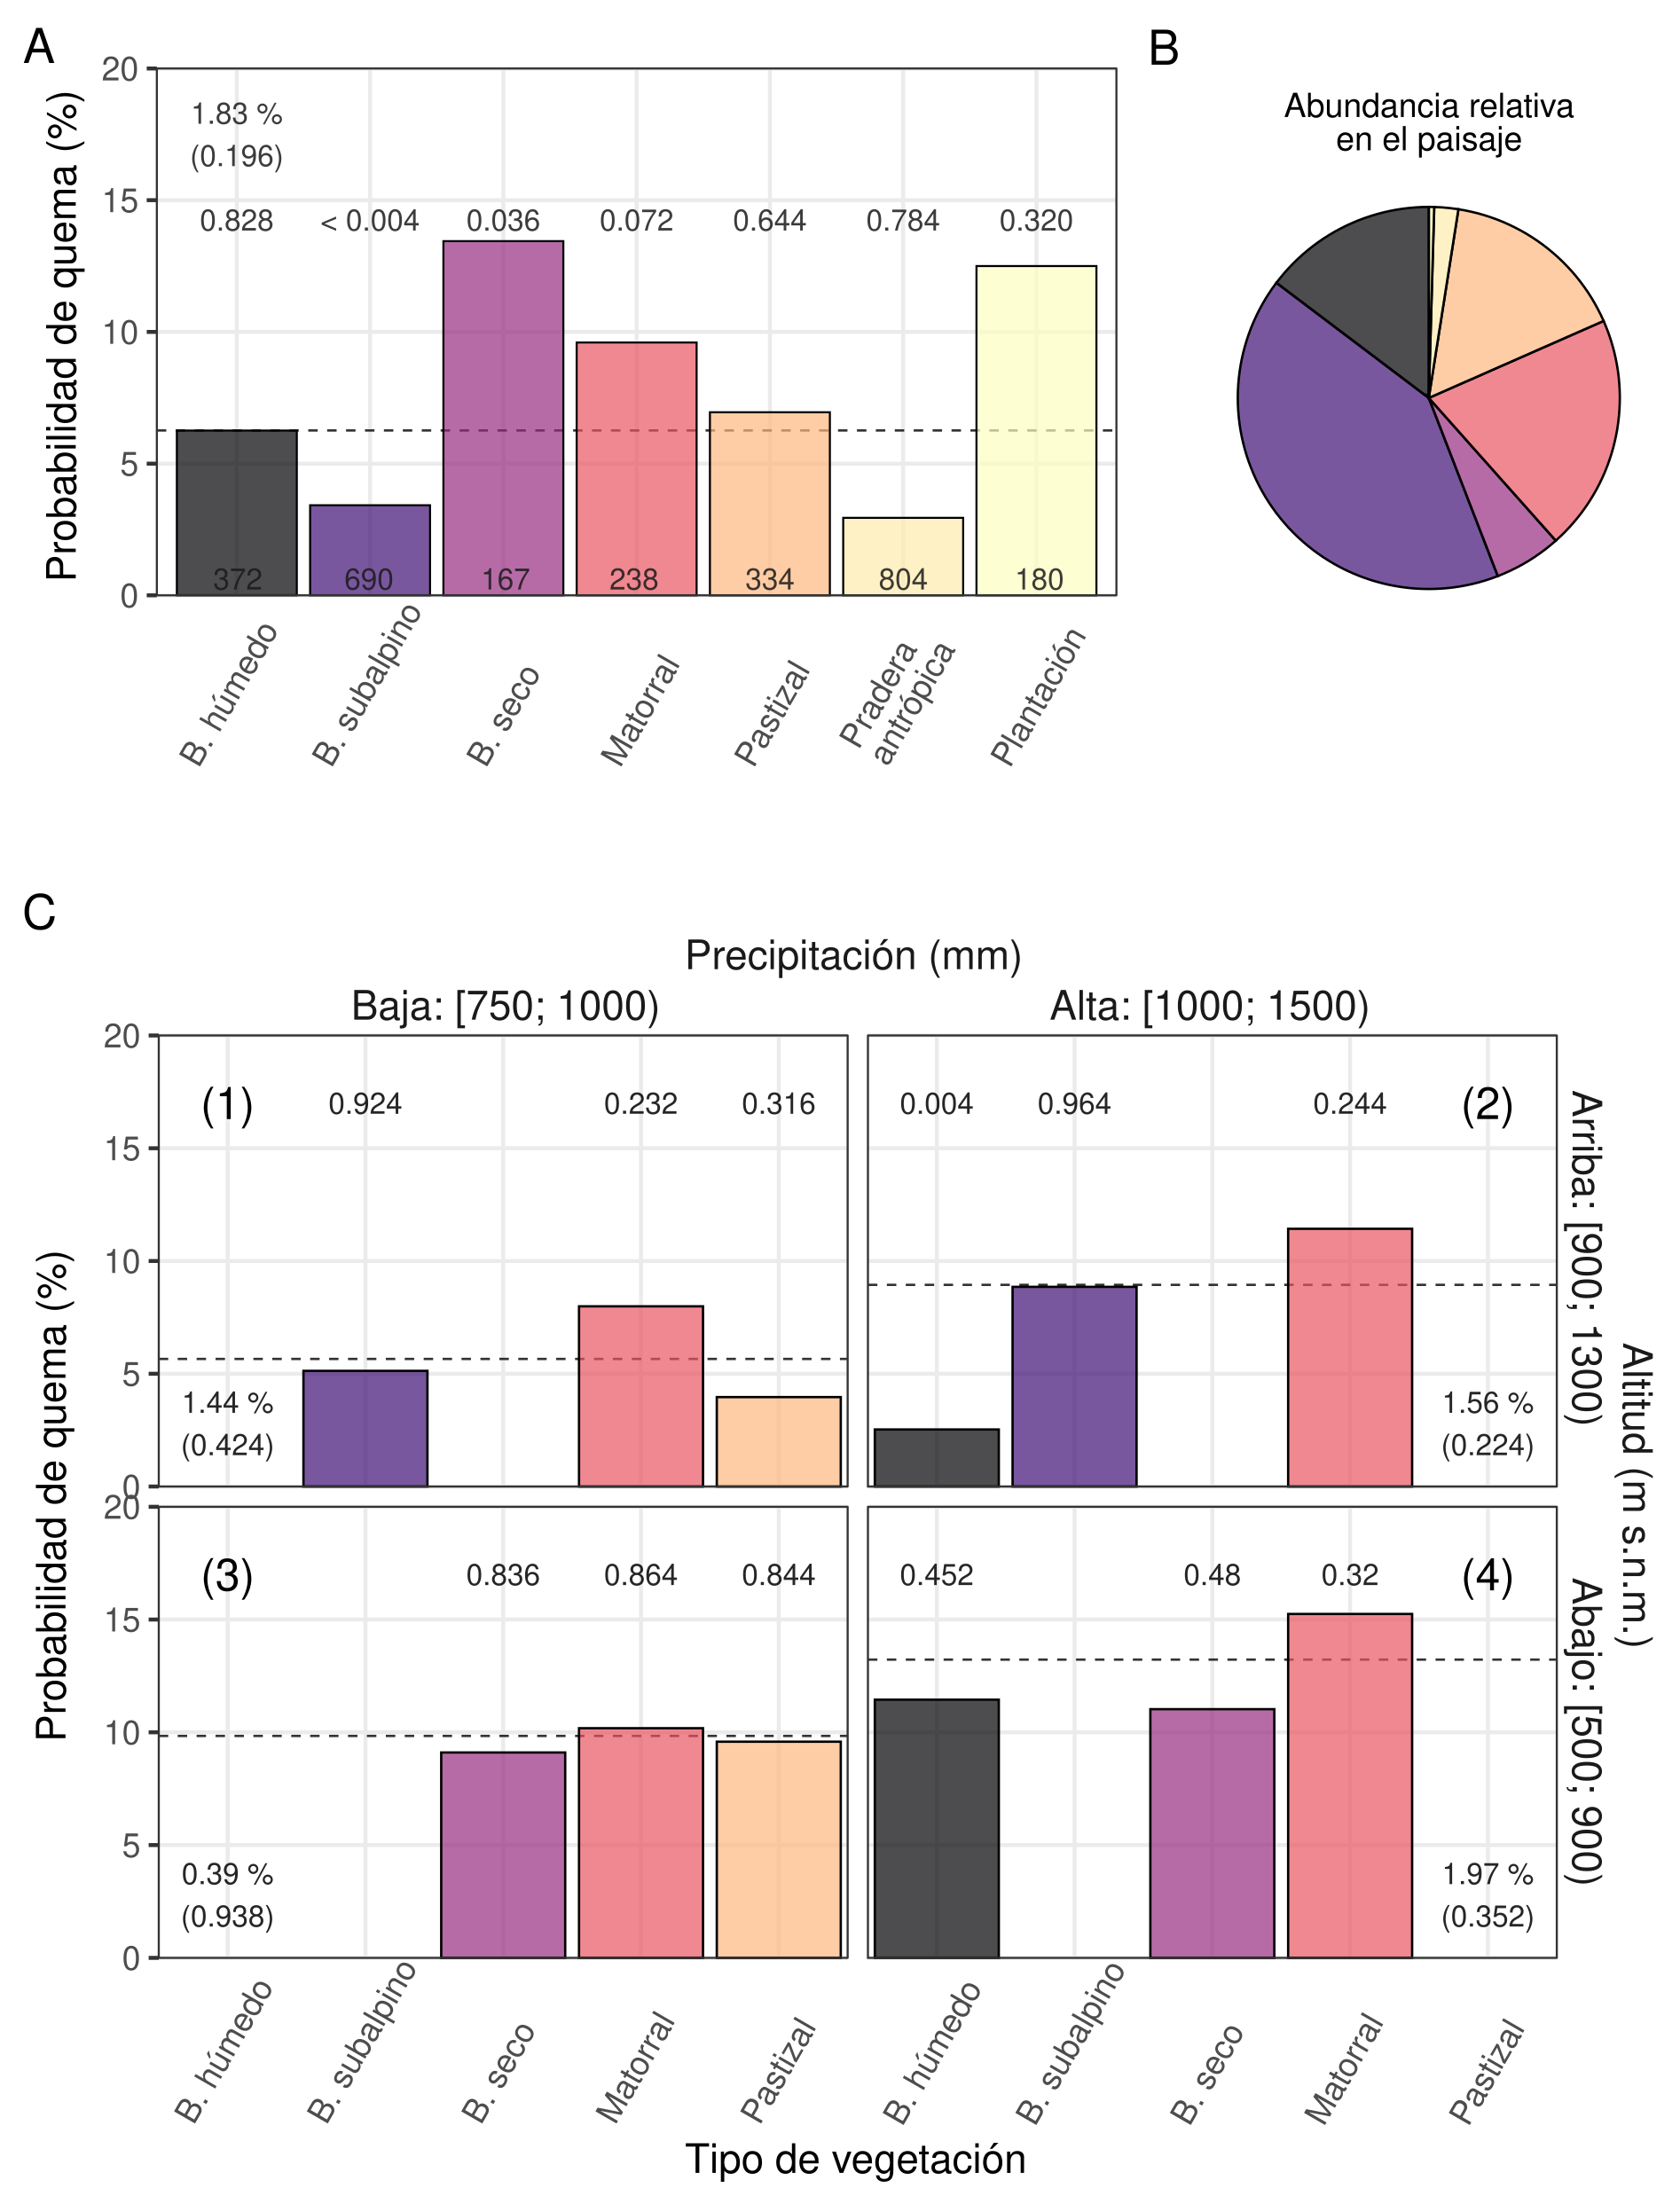
\includegraphics[width=16cm]{figuras/cap3/06) vegetation_v2.png}
    \caption[Probabilidad de quema en función del tipo de vegetación.]{(Leyenda en la página siguiente.)} 
    \label{fig:cap3-06}
\end{figure}

% leyenda en la página siguiente
\begin{figure}[p]
  \contcaption{(en la página anterior). (A) Probabilidad de quema en función del tipo de vegetación, predicha por el modelo de vegetación. En la base de las barras se indica el período de rotación ($PRF$, años), calculado a partir de la probabilidad de quema anual ($p_a$): $PRF = p_a^{-1}$. Dado que modelamos la probabilidad de que las celdas se quemaran al menos una vez en 24 años ($p_{24}$), obtuvimos la probabilidad de quema anual de la siguiente manera: $p_a = 1 - (1 - p_{24}) ^ {1/24}$. (B) Abundancia relativa de cada tipo de vegetación en el área quemable (las plantaciones casi no se distinguen por su baja representatividad en el paisaje). (C) Probabilidad de quema en función del tipo de vegetación, predicha por el modelo conjunto en cuatro condiciones ambientales, como un gráfico de dependencia parcial particionado (Apéndice~\ref{append:veg-comparison}). Algunos tipos no fueron graficados en condiciones ambientales donde es poco probable encontrarlos. En A y C, la línea horizontal discontinua muestra la probabilidad promedio de quema entre los tipos de vegetación ponderada por la abundancia relativa. Los números sobre las barras muestran los valores P a dos colas para las probabilidades de quema (Apéndice~\ref{append:pvalues}), y el porcentaje dentro de cada panel muestra el tamaño del efecto del tipo de vegetación con su correspondiente valor P (Apéndice~\ref{append:effsize}).} 
\end{figure}

% \FloatBarrier

\begin{table}[H]
\centering
\caption[$\text{R}^2$ de los modelos espaciales de probabilidad de quema.]{Valores de $\text{R}^2$ bayesiano \citep{gelman_r-squared_2019} para los tres modelos de probabilidad de quema y métricas de pruebas de razón de verosimilitud que comparan los modelos de vegetación y ambiental con el modelo conjunto. GL: grados de libertad.}
\label{tab:cap3-spat-models}
\begin{tabular}{lcccc}
\toprule
Modelo & $\text{R}^2$ (\%) & $\chi^2$ & GL & P \\
\midrule
Vegetación    & 1.51  & 677.65  & 67.532 & $<$ 2.2E-16 \\
Ambiental     & 8.36  & 249.01  & 56.583 & $<$ 2.2E-16 \\
Conjunto      & 12.73 & -       & -      & -           \\
\bottomrule
\end{tabular}
\end{table}


\FloatBarrier

\section{Discusión}

\subsection{Régimen de incendios}

La proporción quemada anual media, 0.25 \%, presenta una magnitud semejante a la reportada por estudios previos en la región, aunque es ligeramente superior: \citet{paritsis_habitat_2013} reportaron un 0.08 \% para el período 1984-2010, y los parques nacionales en nuestra área de estudio informan un 0.13 \% para el período 1938-1998 (\citealt{bruno_incendios_1982}; APN, datos no publicados). Aunque aparentemente alta y notablemente mayor a lo registrado para mediados del S. XX \citep{Gowda2012}, estos valores son notablemente menores a los estimados para fines del S. XIX y comienzos del S. XX, período en que los colonos euroamericanos usaban el fuego para abrir tierras para la cría de ganado \citep{veblen_historical_2008}. Según el análisis de Veblen et al. \citealt{veblen_historical_2008}, se estima que para el Parque Nacional Nahuel Huapi, entre 1890 y 1914 la tasa media de quema anual fue del 0.92 \%, en base a mapas de \citet{Willis1914}. A su vez, según mapas de \citet{Rothkugel1916}, en las provincias de Neuquén, Río Negro y Chubut, las zonas boscosas se quemaron en una tasa media de 1.48 \% anual en el mismo período. 

En relación a otras regiones, la proporción quemada anual media en nuestra área de estudio entre 1999 y 2022 es aproximadamente un orden de magnitud inferior a la reportada para las sierras del centro de Argentina (1.3-3.2 \%; \citealt{arganaraz_incidencia_2020}), para el Chaco Seco argentino (2.65 \%; \citeauthor{FerroChaco}, en revisión) y para áreas dominadas por coníferas en América del Norte (por ejemplo, 1.7 \%; \citealt{riddle2023wildfire}). La tasa de quema comparativamente baja que encontramos en esta región se asemeja a lo reportado en bosques de especies latifoliadas en el hemisferio norte, que presentan tasas de quema mucho más bajas que los bosques de coníferas \citep{marchal_turning_2020, foster_bottom-up_2022}.

La variación intraanual de la ocurrencia de incendios muestra que, aunque el área quemada alcanza su máximo durante el verano (enero-marzo), los incendios ocurren desde la primavera y aumentan su frecuencia en el verano. Los incendios frecuentes de mediados de verano (enero y febrero), iniciados por humanos o rayos, pueden eventualmente volverse grandes debido a la presencia de combustibles listos para arder (bajo contenido de humedad) combinados con condiciones climáticas que favorecen la propagación del fuego (máximo número de días consecutivos con alta temperatura, baja humedad y/o ausencia de lluvia). Los incendios de primavera, en su mayoría iniciados accidentalmente por humanos, tienden a permanecer pequeños debido a los altos niveles de humedad en la vegetación y condiciones climáticas menos favorables para la propagación del fuego \citep{barbera_microclimate_2023}. En nuestra área de estudio, el área quemada y el número de incendios disminuyen drásticamente cuando comienza el otoño, a pesar de la alta abundancia de especies caducifolias. Al parecer, la abundante precipitación en abril contrarresta los efectos del secado de los combustibles relacionado con la senescencia, lo que contrasta con otros bosques caducifolios que reciben menos precipitación en otoño (e.g., \citealt{tian_wildfires_2011}).

\subsection{Patrones temporales interanuales: incidencia del fuego en función de las variaciones climáticas}

Además del claro patrón estacional, también encontramos efectos marcados de la variabilidad climática interanual sobre la proporción quemada y el número de incendios, mostrando que la actividad del fuego aumenta en años con veranos más secos y cálidos \citep{kitzberger_climatic_1997, kitzberger_influences_1997, holz_ecological_2012, de_torres_curth_incendios_2008, kitzberger_projections_2022}. Otros estudios indican que este efecto se intensifica cuando las sequías comienzan desde el invierno anterior a la temporada de incendios, lo que sugiere un efecto acumulativo del déficit hídrico sobre la humedad del combustible \citep{kitzberger_climatic_1997, kitzberger_influences_1997, de_torres_curth_incendios_2008, kitzberger_projections_2022}. La mayor área quemada durante los veranos cálidos y secos se explica claramente por la humedad de los combustibles, pero dado que la incidencia de rayos aumenta bajo estas condiciones, una mayor tasa de ignición también podría contribuir a este patrón \citep{kitzberger_climatic_1997}. La variabilidad climática interanual también explica en gran medida los patrones de área quemada en otros bosques boreales y templados \citep{gill_top-down_2009, whitlock_past_2015, sommerfeld_patterns_2018, seidl_globally_2020, gaboriau_drivers_2022}.

A pesar del registro relativamente corto, encontramos una tenue tendencia al aumento en la proporción quemada y el número de incendios, similar al patrón encontrado en una serie temporal más larga. Aunque esta tendencia presentó un valor P alto, el aumento en la proporción quemada y el número de incendios coincide con una fase positiva proyectada para la Oscilación Antártica durante el siglo XXI \citep{thompson_signatures_2011}, lo que indica un cambio hacia un clima más favorable para los incendios, evidente también en nuestra serie climática, con una clara tendencia hacia veranos más cálidos y secos. Además, se espera que la probabilidad de incendios bajo escenarios de calentamiento global en el norte de la Patagonia Andina aumente entre 3 y 8 veces respecto a los valores actuales para fines de siglo, dependiendo del escenario climático \citep{kitzberger_projections_2022}. Asimismo, los efectos y tendencias climáticas encontrados en nuestro estudio coinciden con observaciones a nivel global, que asocian una mayor incidencia de incendios con el cambio climático \citep{wang_increasing_2015, robinne_global_2018, ellis_global_2022, lund_influence_2023}. Por lo tanto, la alta incertidumbre en la tendencia creciente de la proporción quemada anual probablemente sea resultado de un bajo poder estadístico. Esta tendencia probablemente se volverá estadísticamente más clara cuando se analicen más años. En particular, los análisis separados de las tendencias del área quemada por incendios causados por rayos y por humanos podrían ayudar a proyectar la incidencia del fuego, ya que ambas causas pueden responder de manera diferente al cambio climático y presentar desafíos contrastantes para el manejo. Se espera que la incidencia de rayos aumente en el norte de la Patagonia Andina con el cambio climático \citep{veblen_historical_2008} y, por lo tanto, la mayor parte del área quemada en el futuro podría ser causa de incendios por rayos, como se ha reportado en otras regiones \citep{miller2012trends, cattau2020anthropogenic}.

\subsection{Patrones espaciales: efectos de la vegetación, topografía, precipitación e influencia humana}

El tipo de vegetación y el entorno físico afectan la ocurrencia de incendios, pero comprender su influencia es desafiante porque el tipo de vegetación varía a lo largo de gradientes ambientales. Aunque estos efectos no pueden aislarse completamente con datos observacionales, nuestro estudio mejoró la comprensión de sus efectos separados sobre los incendios. Encontramos que, aunque la topografía determina en gran medida el tipo de vegetación en el norte de la Patagonia Andina, sus efectos más importantes sobre la actividad de incendios no pueden explicarse únicamente por la variación de los tipos de vegetación a lo largo de los gradientes topográficos. En cambio, la mayoría de sus efectos son evidentes dentro de los distintos tipos de vegetación. Por el contrario, la disminución de la ocurrencia de incendios en zonas de mayor precipitación y en laderas orientadas al sur se explica principalmente por cómo varían los tipos de vegetación con diferente cantidad y continuidad de combustible a lo largo de estos gradientes.

La marcada disminución de la probabilidad de quema con la altitud probablemente resulte de la reducción de la temperatura, lo que disminuye la evapotranspiración y retrasa el secado de los combustibles. De manera similar, la reducción de la probabilidad de quema en áreas con pendientes suaves y ubicadas en posiciones topográficas bajas puede explicarse por la mayor acumulación de agua y menor escorrentía en esos sitios. Dado que estas condiciones promueven una alta humedad de los combustibles, se espera que efectos similares de la topografía se encuentren en todos los tipos de vegetación. Además, las pendientes pronunciadas pueden quemarse más que las áreas planas porque favorecen la propagación del fuego cuesta arriba. Aunque las pendientes empinadas también podrían dificultar la propagación cuesta abajo, ese efecto parece ser menor que la facilitación de la propagación cuesta arriba, lo que explicaría por qué las áreas con mayor pendiente tienden a quemarse más. Este efecto también se espera que opere en todos los tipos de vegetación. Sin embargo, los efectos de la topografía mostraron cierta variación entre los tipos de vegetación. En algunos casos, esta variación se explica por el peso relativo de otras predictoras que covarían con la altitud, pero tienen efectos opuestos. Por ejemplo, en los pastizales, la pendiente y la posición topográfica no afectan la probabilidad de quema porque, al aumentar, también aumenta la altitud, contrarrestando sus efectos por disminuir la temperatura. Pero al controlar por altitud, la pendiente y la posición topográfica más alta aumentan la probabilidad de quema (Apéndice~\ref{append:cov}, Fig.~\ref{fig:cap3-S08}). Un fenómeno similar explica la baja importancia relativa de la altitud en los bosques subalpinos. A mayor altitud, las pendientes se vuelven más pronunciadas y el NDVI disminuye (Fig.~\ref{fig:cap3-S04} y \ref{fig:cap3-S07}A.3), contrarrestando el efecto de la menor temperatura sobre la probabilidad de quema. Nuevamente, al controlar por pendiente y NDVI, la altitud muestra un efecto importante en los bosques subalpinos (Fig.~\ref{fig:cap3-S08}). Sin embargo, en el caso de los matorrales, la baja importancia de la altitud no se explica por efectos contrapuestos de otras predictoras, sino probablemente por su fisonomía. Dado que presentan elevada cantidad y continuidad de combustible fino y un microclima que favorece el secado del combustible \citep{paritsis_positive_2015, tiribelli_changes_2018, barbera_microclimate_2023}, la menor temperatura a mayor altitud probablemente no reduzca tanto su inflamabilidad. Finalmente, los elevados valores P obtenidos para los efectos de la altitud en los bosques secos y matorrales probablemente resulten de la baja abundancia del primero y de la pequeña magnitud de efecto en el segundo, situaciones que reducen el poder estadístico.

A diferencia de los controles topográficos más importantes sobre el fuego, el efecto de la precipitación observado cuando no se consideraron los tipos de vegetación (en el modelo ambiental) parece explicarse principalmente por la variación en los tipos de vegetación a lo largo del gradiente de precipitación (Fig.~\ref{fig:cap3-S01}), y no tanto por cómo la precipitación afecta las condiciones del combustible dentro de los tipos de vegetación. La menor probabilidad de quema encontrada en áreas con alta precipitación probablemente se explique por la alta abundancia de bosques húmedos y subalpinos (Fig.~\ref{fig:cap3-S01}), que tienen baja continuidad vertical del combustible y un sotobosque con humedad intrínsecamente alta \citep{paritsis_positive_2015, tiribelli_changes_2018, barbera_microclimate_2023}. A medida que disminuye la precipitación, el aumento en la cobertura de matorrales parece incrementar la inflamabilidad, ya que presentan mayor cantidad y continuidad de combustible y menor humedad debido a la falta de un dosel cerrado. Sin embargo, en el rango más bajo de precipitación, por debajo de 800 mm / año, la precipitación parece afectar el fuego al controlar los combustibles dentro de los tipos de vegetación. En este rango, donde los pastizales son el tipo de vegetación dominante (Fig.~\ref{fig:cap3-S01}), la probabilidad de quema decae con la disminución de la precipitación (Fig.~\ref{fig:cap3-05}A.1). Por lo tanto, esa disminución en la probabilidad de quema ocurre porque los pastizales presentan menor productividad a baja precipitación (Fig.~\ref{fig:cap3-S07}E.6), y el fuego está limitado por la continuidad del combustible.

Encontramos que las diferencias en la probabilidad de quema entre los tipos de vegetación se explican tanto por su cantidad y continuidad de combustible contrastantes como por las condiciones topográficas donde cada uno es más abundante. La baja y alta probabilidad de quema encontradas en los bosques subalpinos y secos, respectivamente, cuando no se consideraron las predictoras ambientales, se explican en gran medida porque ocurren en los rangos de altitud más altos y más bajos. Al compararlos con otros tipos de vegetación a iguales condiciones, los bosques secos mostraron una probabilidad de quema relativamente baja, y los bosques subalpinos, valores intermedios. Para los bosques subalpinos esperábamos encontrar una probabilidad de quema similar a la de los bosques húmedos, debido a su similitud estructural, pero mostraron una probabilidad mayor. Esto podría explicarse por que las lengas presentan menor altura que los coihues, confiriendo una mayor continuidad vertical del combustible a los bosques subalpinos en comparación con los húmedos.

Nuestros resultados coinciden con la hipótesis de restricciones variables, donde las áreas de productividad intermedia muestran la mayor probabilidad de quema \citep{pausas_global_2013, krawchuk_constraints_2011}, en concordancia con \citet{kitzberger_projections_2022}. Este patrón también fue evidente dentro de los tipos de vegetación, y nuestros resultados sugieren que los bosques húmedos y subalpinos de baja productividad podrían presentar incluso mayor probabilidad de quema que los matorrales. Estos bosques con NDVI relativamente bajo ($\approx$~0.7) probablemente sean aquellos con doseles abiertos, donde la cantidad de combustible es alta y la humedad del combustible es baja. En los matorrales, el NDVI mostró efectos menores sobre la probabilidad de quema en comparación con la mayoría de los otros tipos de vegetación, lo que sugiere que, a pesar de presentar variabilidad en la cantidad y continuidad de combustible, rara vez alcanzan condiciones que reduzcan marcadamente la probabilidad de quema, ya que rara vez presentan doseles cerrados y altos. 

Dada la notable importancia de la productividad sobre la inflamabilidad de bosques y pastizales, será necesario evaluar cómo el cambio climático puede alterarla. En algunas regiones, el cambio climático aumenta la productividad debido a la mayor concentración de $\text{CO}_2$ atmosférico \citep{silva2013probing,sperlich2020gains}. Sin embargo, en esta región, es probable que el aumento de la temperatura y la disminución de la precipitación sobrecompense este efecto \citep{gutierrez2014increased}. Ante estas condiciones sería esperable que los bosques presenten mayor muerte parcial de copa, mortalidad, y que se vuelvan más abiertos  \citep{suarez2004factors,rodriguez2016influence,molowny2017changes}, lo que aumentaría su inflamabilidad. En caso de que el mismo proceso disminuya la productividad de los pastizales o de los bosques actualmente poco productivos, la inflamabilidad podría disminuir asociada a una menor continuidad del combustible.

A diferencia de los claros efectos de la vegetación y la topografía sobre la ocurrencia de incendios, encontramos un efecto poco claro de la distancia a poblados y a caminos. Sin embargo, el aumento en la probabilidad de quema a mayores distancias, aunque altamente esperado por azar, también podría resultar de incendios causados por rayos, que, al originarse lejos de poblados y caminos, presentan menor probabilidad de ser detectados y controlados. Estudios que analicen por separado las igniciones y la propagación del fuego, considerando la fuente de ignición (rayos vs. humanos), son necesarios para comprender mejor los efectos humanos sobre el fuego (e.g., \citealt{mundo_environmental_2013, morales_stochastic_2015, godoy_forty_2022}).

Nuestro análisis mejoró la comprensión de los efectos separados de la vegetación y las variables ambientales sobre el fuego, aunque reconocemos que este enfoque observacional no puede aislarlos completamente. Específicamente, nuestros resultados destacaron diferencias en la probabilidad de quema entre tipos de vegetación que probablemente sean el resultado de propiedades contrastantes del combustible (Fig.~\ref{fig:cap3-06}C) más que de la variación ambiental. Sin embargo, las diferencias observadas entre tipos de vegetación, incluso cuando se controlan los factores ambientales (Fig.~\ref{fig:cap3-06}C), podrían estar parcialmente influenciadas por variables ambientales no observadas (e.g., humedad del suelo). En general, nuestro estudio proporciona una base para investigaciones de campo más detalladas que permitan refinar nuestra comprensión de los controles del fuego relacionados con la vegetación y variables ambientales.

Los modelos de probabilidad de quema (de vegetación, ambiental y conjunto) presentaron valores de $R^2$ de muy bajos a bajos, lo cual resulta esperable considerando que sólo se utilizaron variables espaciales y no dinámicas. Que un píxel se queme o no depende fuertemente de que ocurra una ignición relativamente cerca o que el fuego propague desde un punto de ignición. Todo este proceso es altamente estocástico, dependiendo de variables meteorológicas y relaciones espaciales (e.g., dirección del viento en relación a las celdas receptora y dadora de fuego) que se resuelven a una escala espacial y temporal fina. Aún así, notamos que existe una marcada variabilidad espacial en la incidencia del fuego que podría ser explicada por variables espaciales asociadas al uso antrópico del territorio. La región Centro-Sur mostró la probabilidad de quema más alta, y la Norte, la más baja (Fig.~\ref{fig:cap3-01}A, Tabla~\ref{tab:cap3-spatvar}). Este patrón podrían ser explicado por diferencias en el manejo del fuego. Por ejemplo, las regiones Centro-Norte y Norte incluyen extensos parques nacionales (Nahuel Huapi y Lanín), en donde la menor incidencia del fuego podría explicarse por mayores esfuerzos de prevención y control. Futuros estudios considerando aspectos de manejo del fuego y otras variables de índole antrópico, como la densidad poblacional, contribuirán a entender mejor esta variabilidad regional. 

Otro aspecto a resaltar en relación a la variabilidad espacial en la incidencia del fuego es que nuestros resultados en cuanto a patrones espaciales pueden estar fuertemente influenciados por las zonas de mayor incidencia del fuego. En este trabajo suponemos los controles espaciales del fuego son similares entre regiones, ya que no tenemos evidencia para suponer diferencias muy marcadas entre ellas. A su vez, decidimos no analizar por separado cada región porque en nuestra área de estudio la incidencia del fuego es baja, y nuestro registro es relativamente acotado en el tiempo. En este contexto, pocos incendios pueden determinar los patrones obtenidos, por lo que se requiere compensar la baja incidencia del fuego y la corta serie temporal analizando grandes áreas. En caso de subdividir el análisis, los patrones se volverían menos confiables. La misma lógica aplica al análisis de la variabilidad interanual en la incidencia del fuego. Puede ocurrir que la tendencia no sea homogénea en el área de estudio, pero con las características de nuestra base de datos no resulta confiable analizar su variación espacial. A futuro, contando con series más largas, podremos analizar en mayor detalle cómo los controles del fuego y su tendencia temporal varían entre regiones.

\subsection{Implicancias para el manejo del fuego}

En ecosistemas donde la inflamabilidad aumenta con el tiempo desde el último incendio, como en los bosques de coníferas del hemisferio norte, los incendios frecuentes y de baja severidad limitan la ocurrencia de incendios extremadamente grandes y severos \citep{ryan_prescribed_2013}. Sin embargo, si (1) la inflamabilidad es mayor en los estadios sucesionales tempranos que en los tardíos, o (2) los tipos de vegetación resilientes al fuego son más inflamables que los sensibles al fuego, agregar fuego al sistema puede promover aún más incendios \citep{kitzberger_decreases_2012, tiribelli_non-additive_2019}. La vegetación del norte de la Patagonia Andina cumple con ambas condiciones. Los bosques, que en promedio son la comunidad menos inflamable, presentan mayor inflamabilidad en su estado sucesional temprano, y esta disminuye desde los 30 años luego de un incendio \citep{tiribelli_changes_2018, tiribelli_non-additive_2019, barbera_microclimate_2023}. A su vez, su regeneración posfuego es limitada \citep{cuevas_tree_2000, kitzberger_effects_2005, tercero-bucardo_field_2007, landesmann_importance_2018}. Los matorrales, más inflamables, persisten después del fuego y frecuentemente reemplazan a los bosques quemados \citep{kitzberger_firevegetation_2016, landesmann_increased_2021}. Estas dinámicas resultan en un ciclo donde el fuego frecuente promueve vegetación más inflamable, lo que a su vez promueve más incendios. Por lo tanto, para reducir los impactos del fuego en la sociedad y los ecosistemas, que se espera que aumenten con el cambio climático, es necesario limitar la ocurrencia de incendios tanto como sea posible.

Encontramos que las comunidades leñosas más productivas tienden a quemarse menos. Aunque la baja probabilidad de quema en áreas de alto NDVI puede deberse a la alta disponibilidad de agua relacionada con condiciones físicas a pequeña escala (e.g., alta humedad del suelo, menor insolación), esto también podría reflejar una estructura particular de la vegetación. Las áreas de alta productividad usualmente presentan doseles altos y cerrados, con sotobosques de escasa biomasa, baja continuidad vertical del combustible y/o alta humedad del combustible. Por lo tanto, promover el crecimiento de árboles altos para crear doseles cerrados que aumenten la humedad del combustible y reducir la cantidad y continuidad de los combustibles en los sotobosques podría reducir significativamente la inflamabilidad. Los doseles altos y cerrados pueden inducirse mediante prácticas de manejo de matorrales, como podar árboles cortos de múltiples tallos (como radales o ñires) para que tengan un solo fuste y así promover el crecimiento vertical, o plantar árboles de coihue, lenga y ciprés en la matriz de matorrales. Los combustibles en el sotobosque podrían reducirse combinando la extracción de leña y madera con la cría de ganado, que muestra un valor económico prometedor \citep{peri_review_2016, goldenberg_efecto_2018, goldenberg_shrubland_2021}. Sin embargo, dado que la humedad del combustible fino también puede disminuir con la cosecha, se necesitan estrategias cuidadosas para disminuir efectivamente la inflamabilidad \citep{goldenberg_effects_2020}. 

% Plantaciones: quitado por sugerencia de Grau, pero mencionar en Cap 5

%Otro aspecto a tener en cuenta en relación al manejo de la vegetación son las plantaciones e invasiones de coníferas exóticas. En la región, numerosas plantaciones de coníferas (\textit{Pinus ponderosa}, \textit{Pinus contorta}, \textit{Pseudotsuga menziesii} y \textit{Pinus radiata}) fueron establecidas desde la década de 1950, y careciendo de un manejo adecuado han acumulado una gran cantidad de combustible, volviéndose altamente inflamables \citep{SAGPyA2017}. A su vez, estas plantaciones son focos de invasión de ecosistemas nativos. Dada la mayor inflamabilidad de las plantaciones de coníferas y los sitios que invaden en comparación con las comunidades nativas \citep{paritsis_pine_2018, franzese_legacy_2022, cingolani2023enrichment}, realizar un manejo adecuado de las mismas mediante raleo y poda, y controlar las invasiones, es de gran importancia para reducir la inflamabilidad del paisaje \citep{gomez-gonzalez2024afforestation}. 

Pero más allá de las estrategias de manejo que pueden disminuir la inflamabilidad del paisaje, se espera que el clima futuro genere incendios que probablemente se propaguen incluso en estos entornos menos inflamables \citep{cawson_atmospheric_2024}, lo que pone en duda la eficacia de la gestión de combustibles como única estrategia. Por lo tanto, reducir las igniciones humanas y generar sistemas más efectivos de detección temprana de incendios podría ser la estrategia más efectiva para reducir la vulnerabilidad al fuego en esta región. Finalmente, las predicciones de modelos de propagación de incendios pueden ser útiles durante el proceso de supresión. Este estudio señala direcciones para mejorar el desempeño de los modelos de propagación recientemente desarrollados en la región \citep{morales_stochastic_2015, laneri_first_2020}, incorporando variables como altitud, NDVI y tipo de vegetación.

\subsection{Conclusiones}

Nuestros resultados confirman el fuerte efecto de la variación climática interanual en la ocurrencia de incendios en el norte de la Patagonia Andina, y también sugieren que el cambio climático aumentará la actividad de incendios, en concordancia con investigaciones previas \citep{kitzberger_projections_2022}. Espacialmente, encontramos que el efecto de la topografía en la ocurrencia de incendios no puede explicarse por la variación en los tipos de vegetación a lo largo de los gradientes topográficos. En cambio, la topografía probablemente afecta el fuego principalmente a través de su efecto en el balance hídrico y, por ende, en el contenido de humedad del combustible, con un efecto similar en todos los tipos de vegetación. Por el contrario, el efecto de la precipitación anual media en la incidencia del fuego se explica por la ocurrencia de tipos de vegetación con cantidad, continuidad y humedad de combustibles finos contrastantes a lo largo del gradiente.

Nuestra descripción de los patrones de área quemada para el inicio del siglo XXI puede servir como un punto de referencia para detectar cambios en el régimen de incendios en la región, y nuestro algoritmo de mapeo de incendios puede usarse para mantener este registro actualizado. Además, una mejor comprensión de cómo el fuego responde a factores biofísicos y humanos podría lograrse estudiando por separado la ignición y la propagación del fuego, para lo cual nuestros resultados y base de datos proporcionan un valioso punto de partida.

\section*{Disponibilidad de datos}

Los datos y el código para reproducir todos los análisis y figuras están alojados en GitHub (\url{https://github.com/barberaivan/patagonian_fires.git}).